\documentclass[../MasterThesis.tex]{subfiles}
\graphicspath{ {./assets/images/} }


%----------------------------------------------------------------------------
%----------------------------------------------------------------------------

\begin{document}
	
	
	
%
%
%
%
%=======================================================================================================
%
%
%
%
%=======================================================================================================
% CHAPTER: DESIGN AND IMPLEMENTATION
%=======================================================================================================
\newpage
\section{Design and Implementation} \label{section:designandimplementation}

In this Chapter, the system architecture and the implementation are explained. First a brief overview of the architecture is given in Section~\ref{subsection:architecturedesign} and then the frontend and backend are described in more detail (Section~\ref{subsection:accuratevideo} and Section~\ref{subsection:jit-webrtc}).
For the application of a MLT filter, different filters were compared to select the most suitable option in Section~\ref{subsection:meltfilter}. Finally, the implementation is described with examples and code excerpts in Section~\ref{subsection:implementation}.





%-------------------------------------------------------------------------------------------------------
\subsection{Architecture Design} \label{subsection:architecturedesign}


The system consists of four components: The frontend that is displayed in the browser, \texttt{main.py} as the Python backend, the MLT framework and a session service. The frontend is described in Section~\ref{subsection:accuratevideo} and the backend components (\texttt{main.py}, the MLT framework and session service) will be described in more detail in Section~\ref{subsection:jit-webrtc}. The structure and usage of MLT was introduced in Section~\ref{subsection:melt}.

% In those Sections, the functionality of the system before the implementation of the colour grading is described. The implementation is described in Section~\ref{subsection:implementation}.

The system architecture can be seen in Figure~\ref{figure:SA}.
A session is initiated through the browser with the session service, which initiates the \texttt{main.py} script.
The Python backend communicates with the MLT framework to use its video editing, processing and transcoding functionalities. The real-time communication is implemented through a WebRTC channel.




\begin{figure}[H]
	\centering
	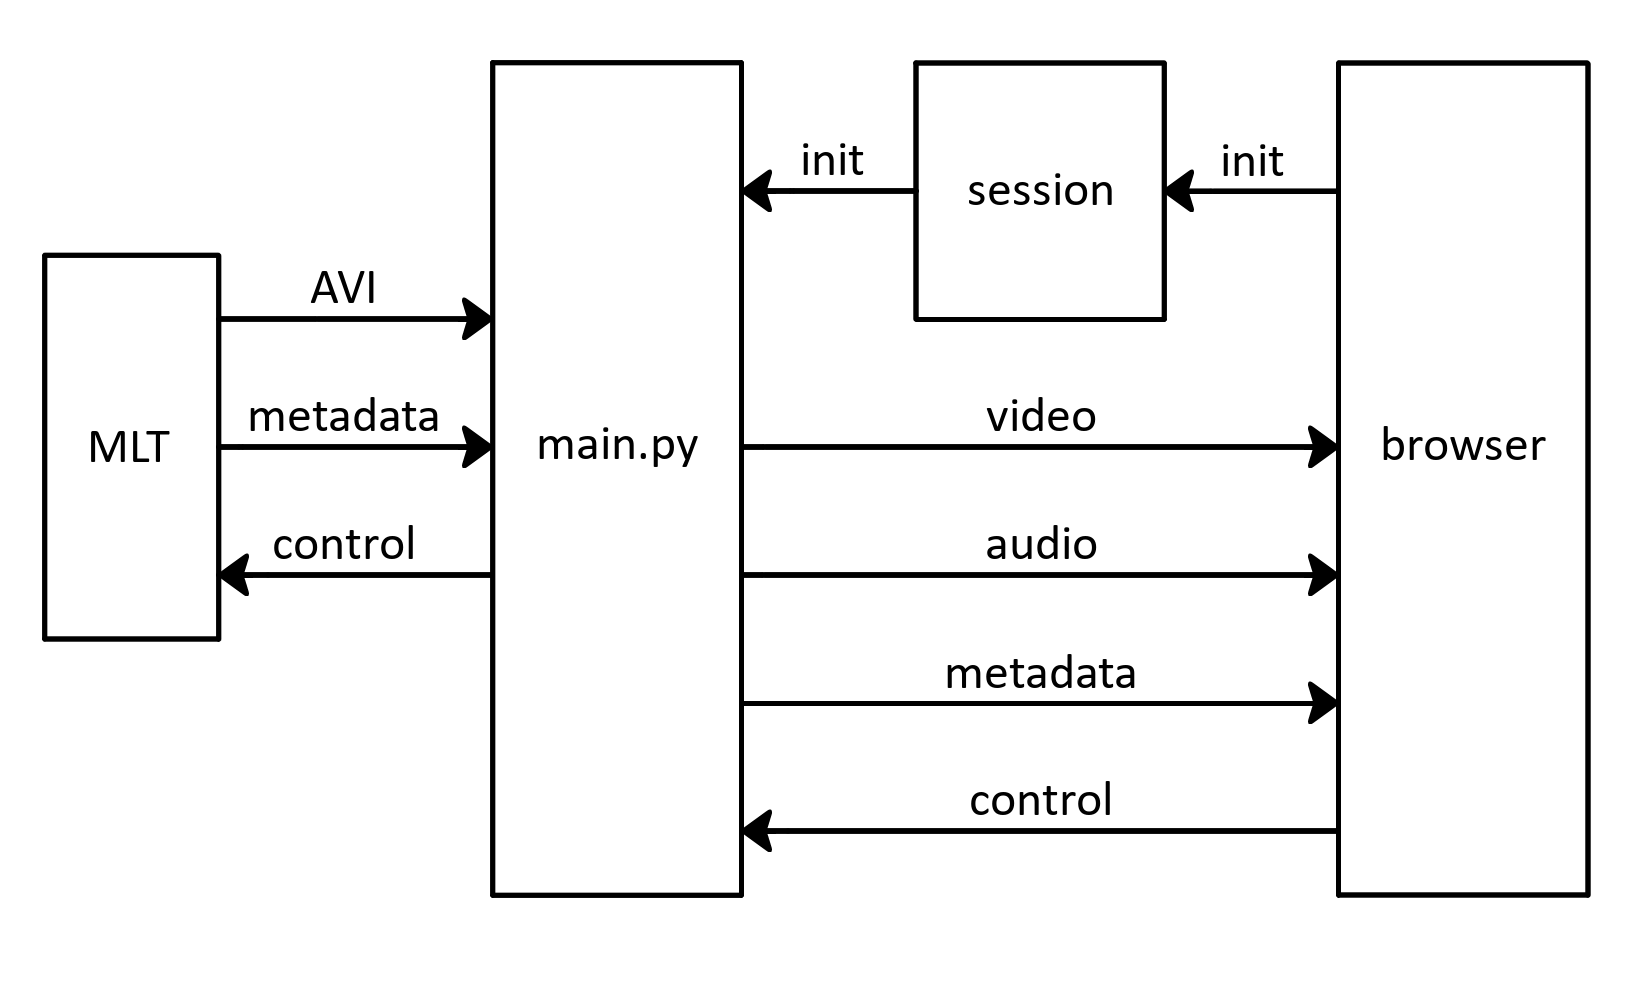
\includegraphics[width=0.8\textwidth]{IM3.png}
	\caption[Architecture of the system that consists of four parts.]{Architecture of the system that consists of four parts.}
	\label{figure:SA}
\end{figure}


For development and testing without the session service, the backend can be started in a Docker container. This has been done for the implementation for this thesis project.







%-------------------------------------------------------------------------------------------------------
\subsection{Accurate Video} \label{subsection:accuratevideo}
% Describe the frontend

The following description of the system is based on the code base and the information from the \texttt{README} file~\cite{RM_Frontend}.
%
The frontend is displayed in the browser and uses Node.js as its runtime environment with Yarn to manage project dependencies and packages. It is developed using HyperText Markup Language (HTML), Cascading Style Sheets (CSS) and JavaScript (JS) to create the user interface.


\begin{figure}[H]
	\centering
	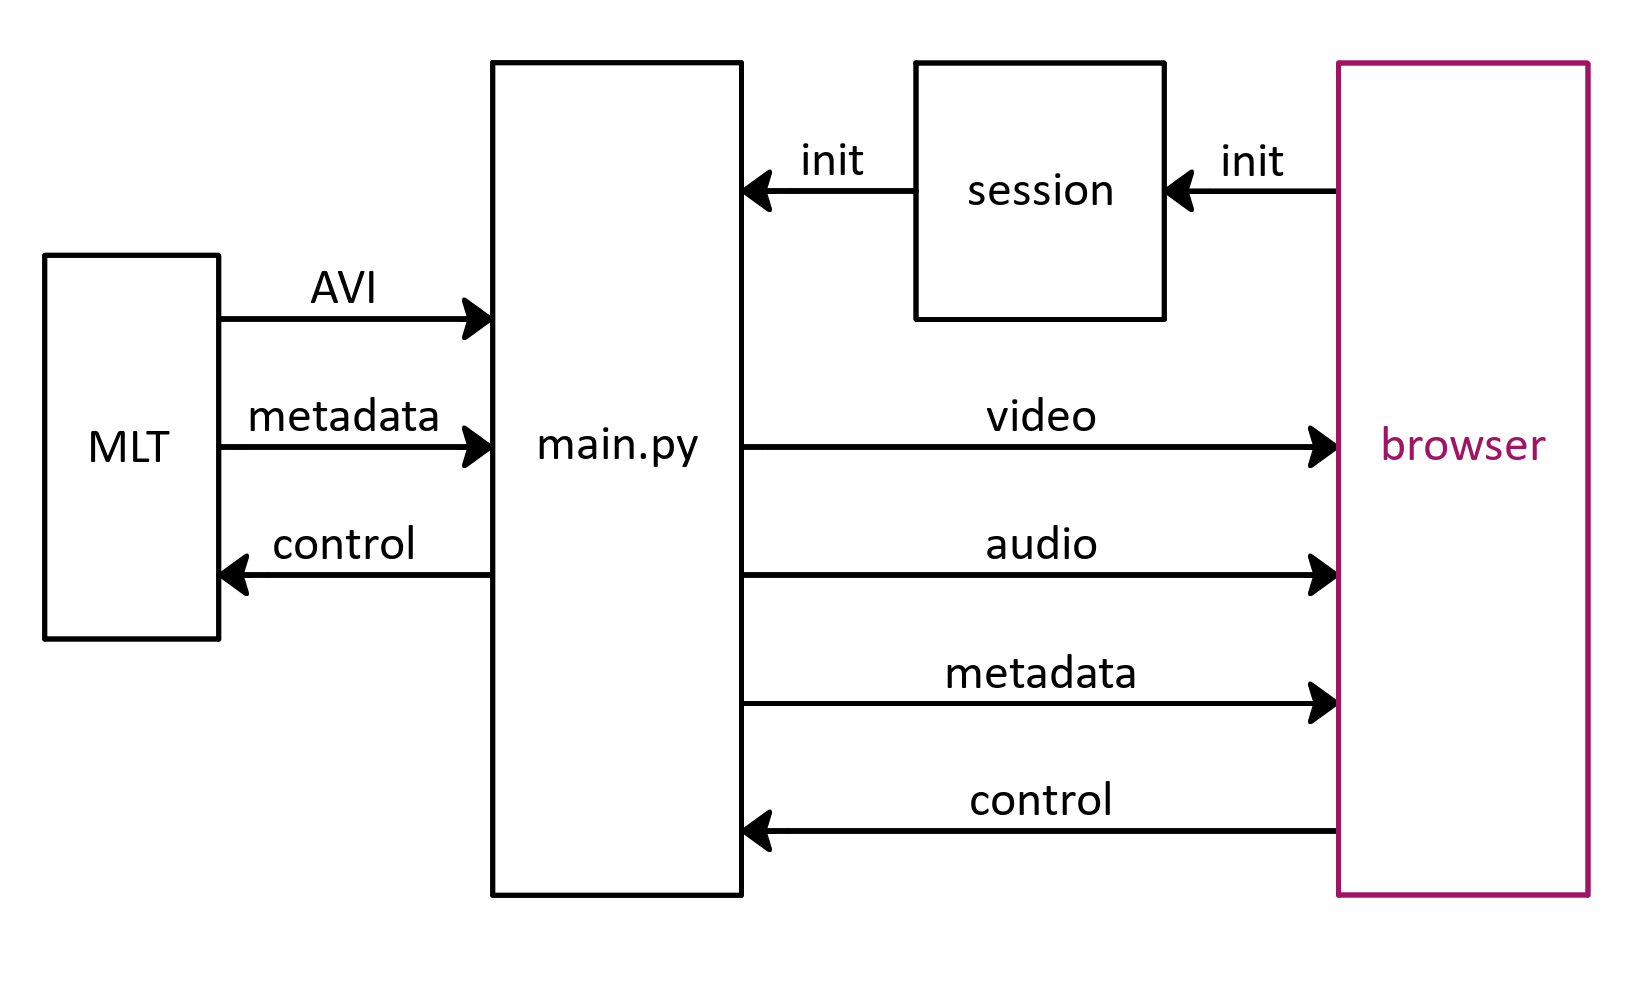
\includegraphics[width=0.5\textwidth]{IM_FE.png}
	\caption{Accurate Video in the system architecture.}
	\label{figure:AS_frontend}
\end{figure}


\hypersetup{urlcolor=black}
The user interface when playing a video in the Accurate Player can be seen in Figure~\ref{figure:AV_before}. This can be found under \url{http://localhost:5000/controls/jit/index.html} when executing the code as described in Section~\ref{subsection:runninghtecode}.
First, a yellow field can be seen (shown on the left in Figure~\ref{figure:AV_before}). After clicking this, a loading screen is displayed (in the middle in Figure~\ref{figure:AV_before}) and then the video can be started by clicking on the play button. The playing of a video can be seen on the right in Figure~\ref{figure:AV_before}.


\begin{figure}[H]
	\begin{center}
		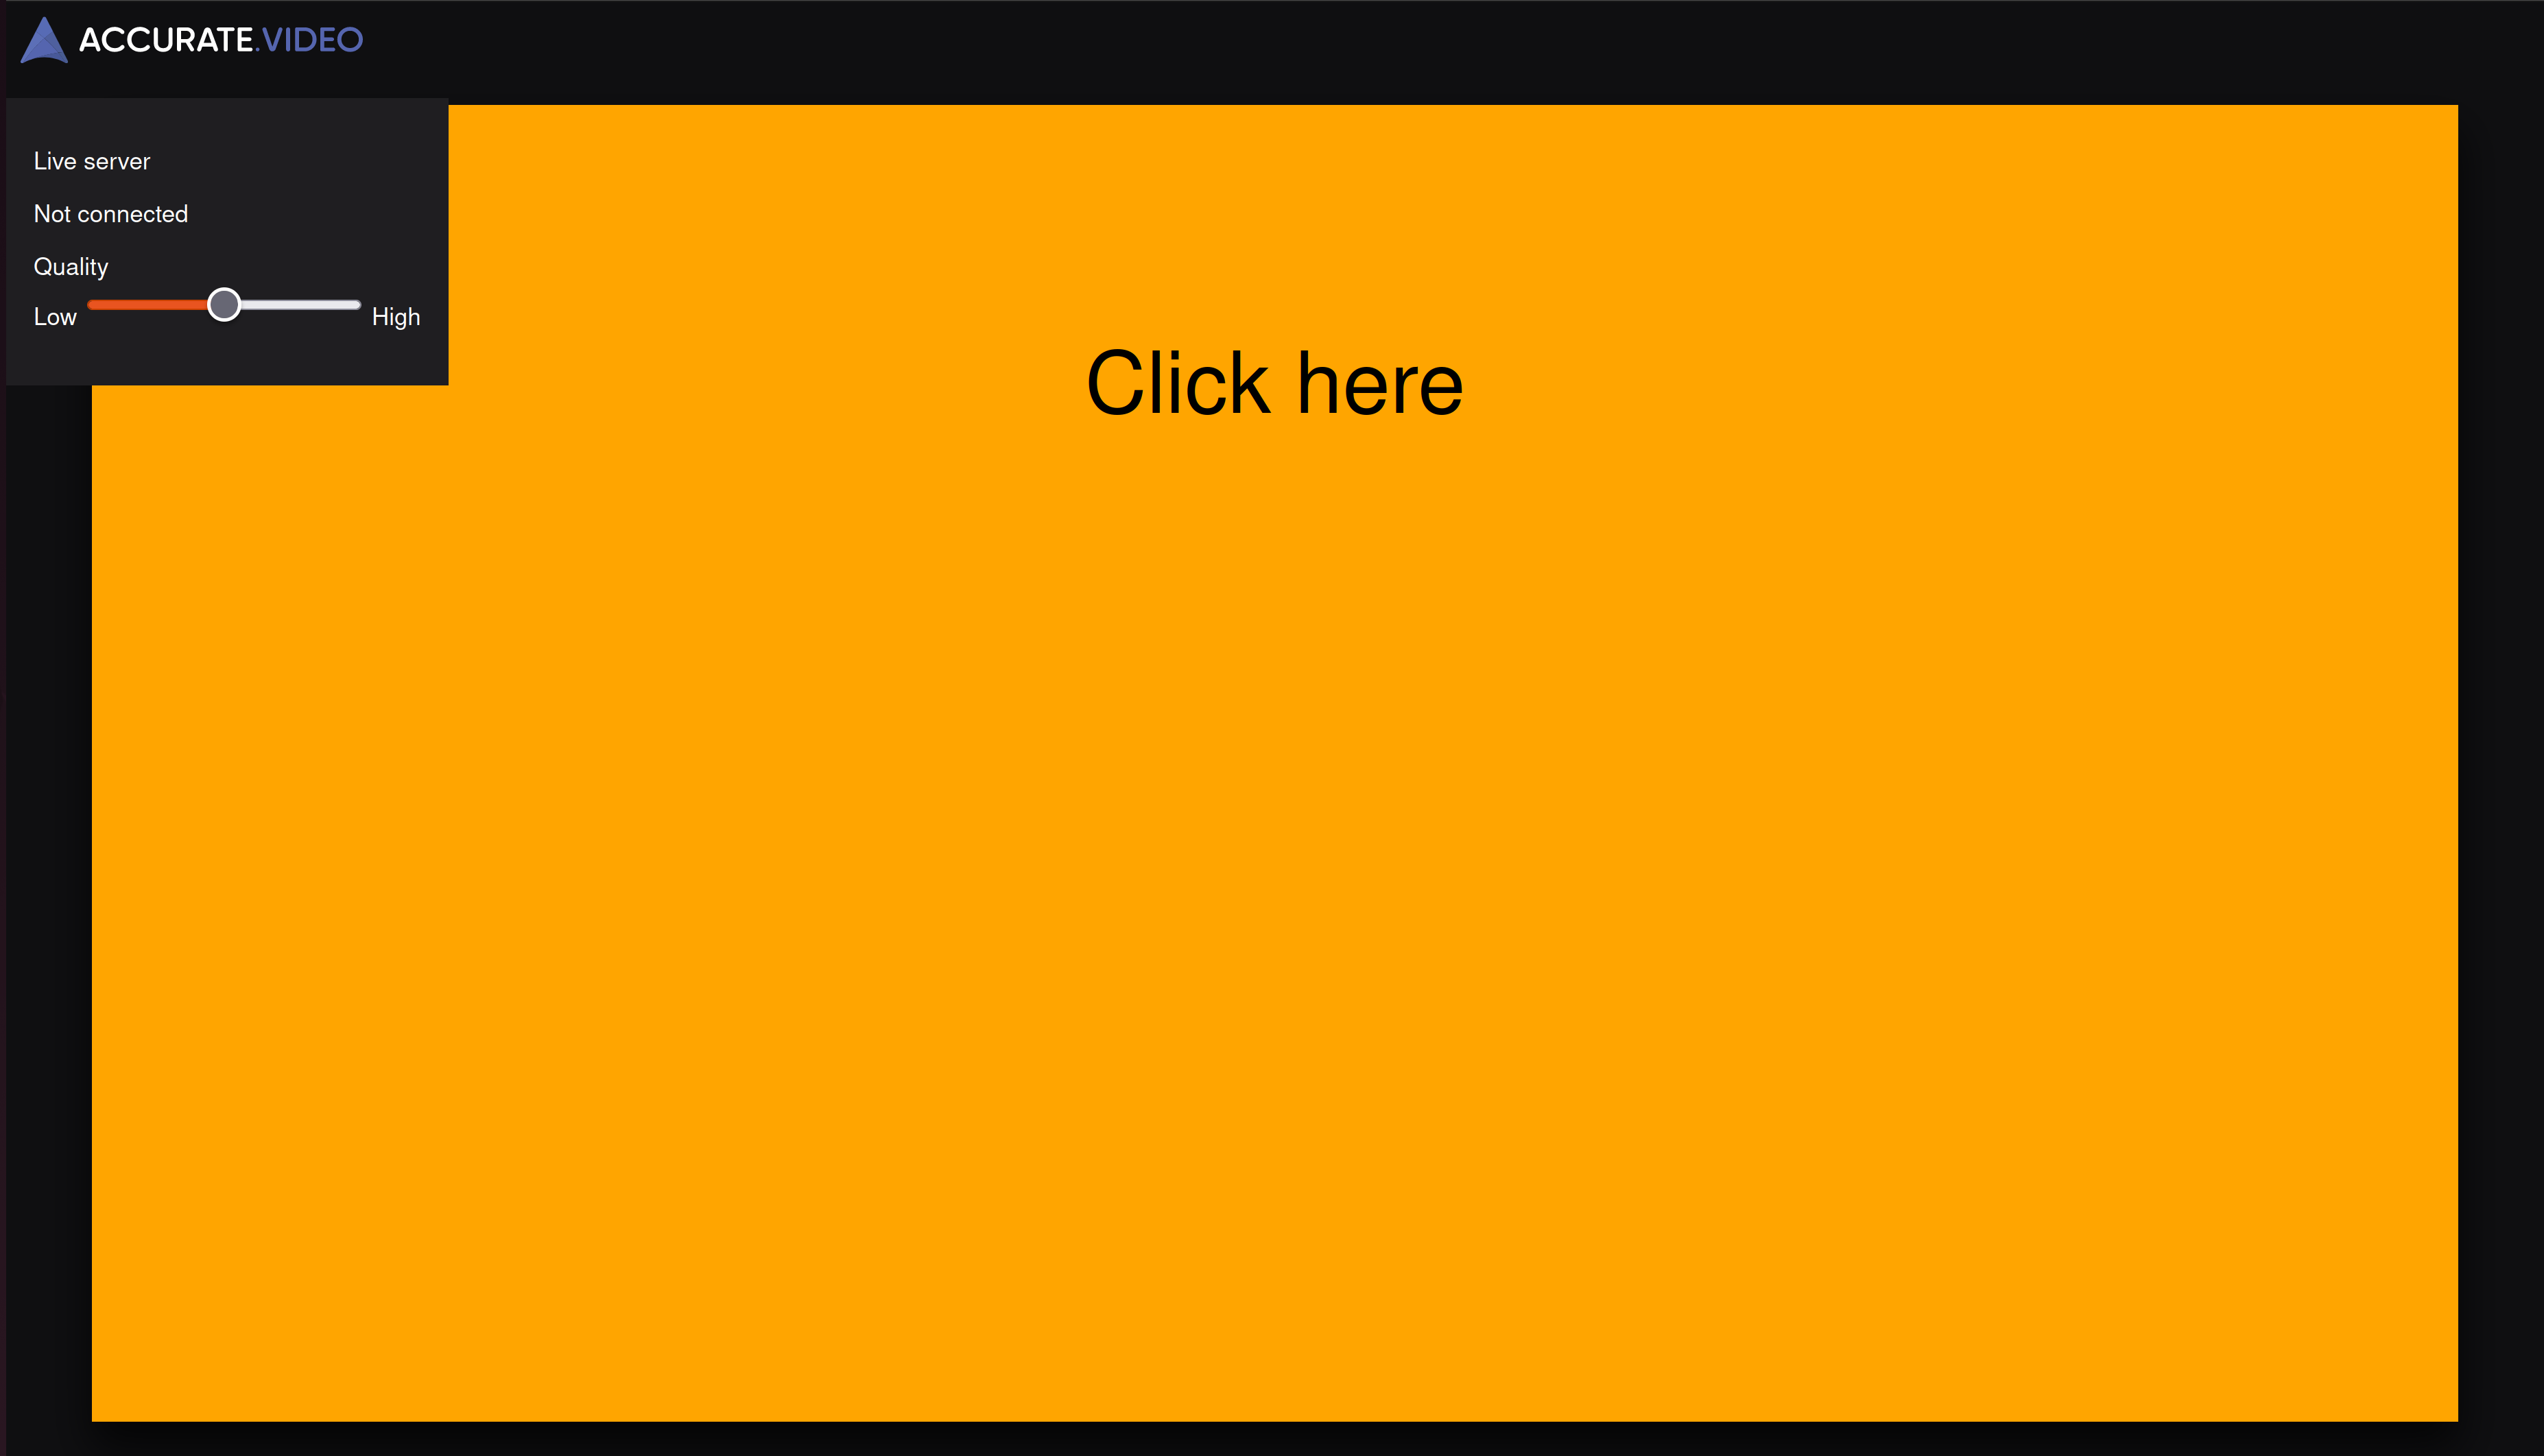
\includegraphics[width=0.32\textwidth]{AV1_before.png} \ 
		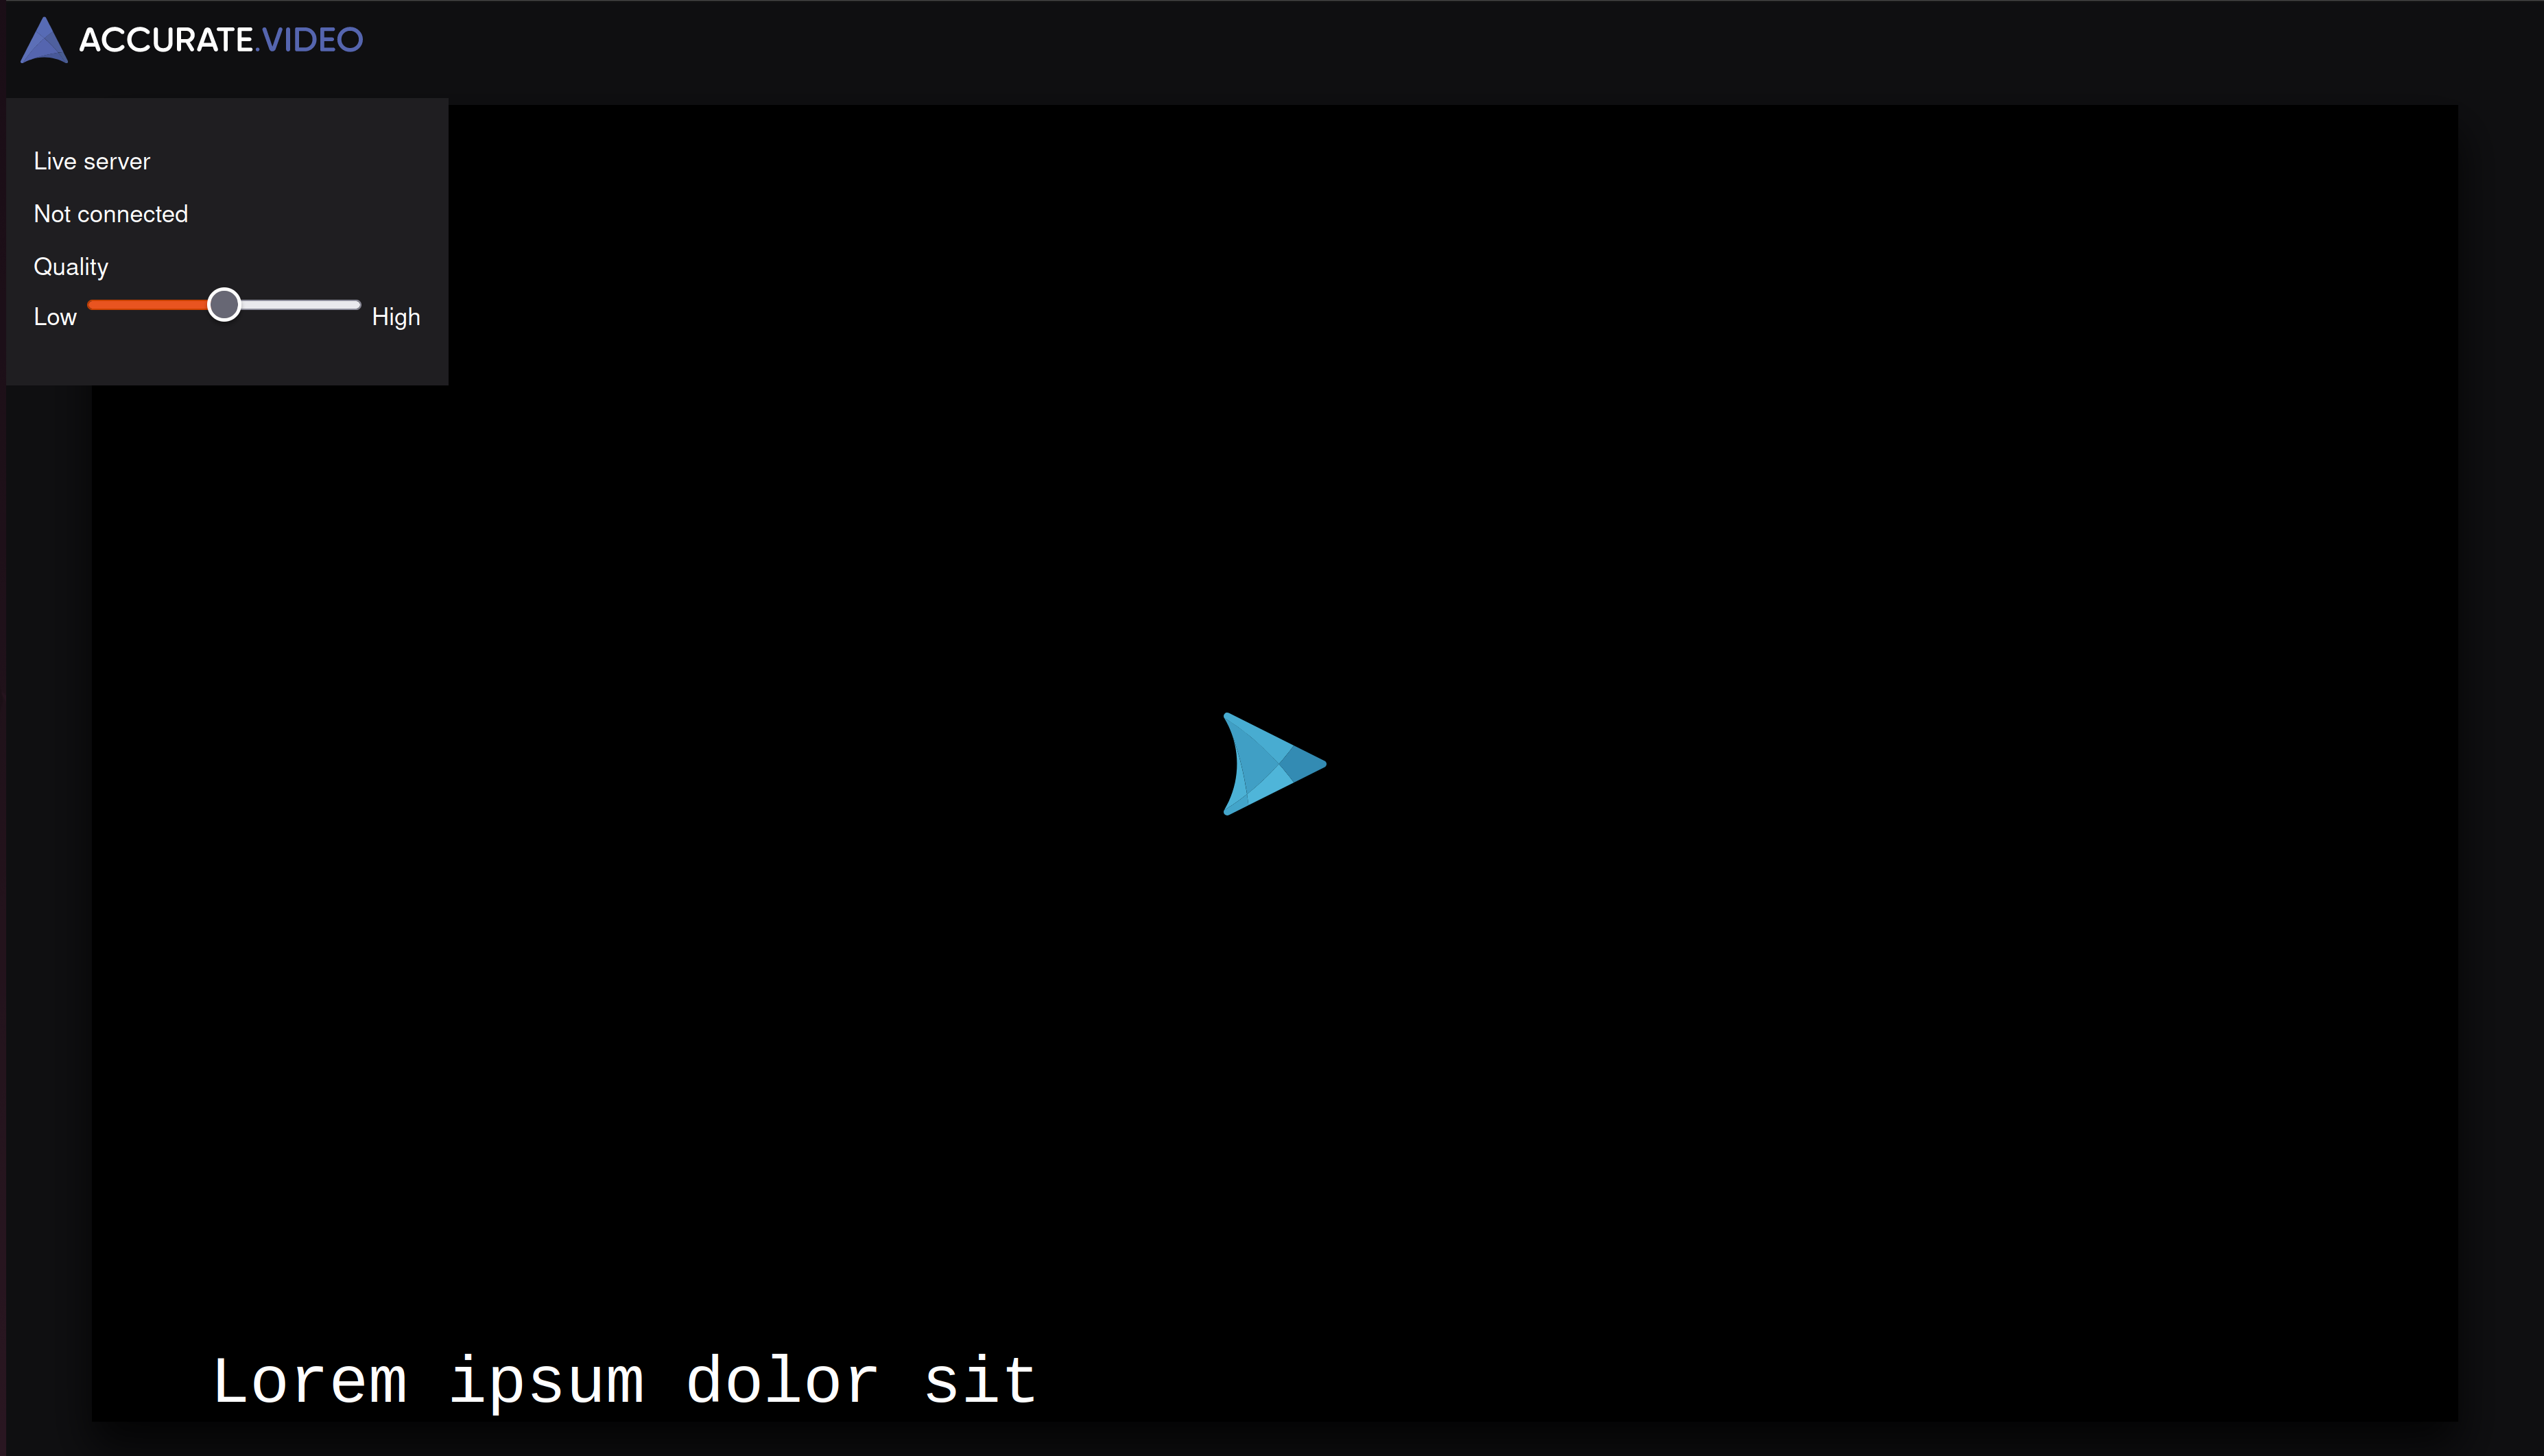
\includegraphics[width=0.32\textwidth]{AV2_before.png} \ 
		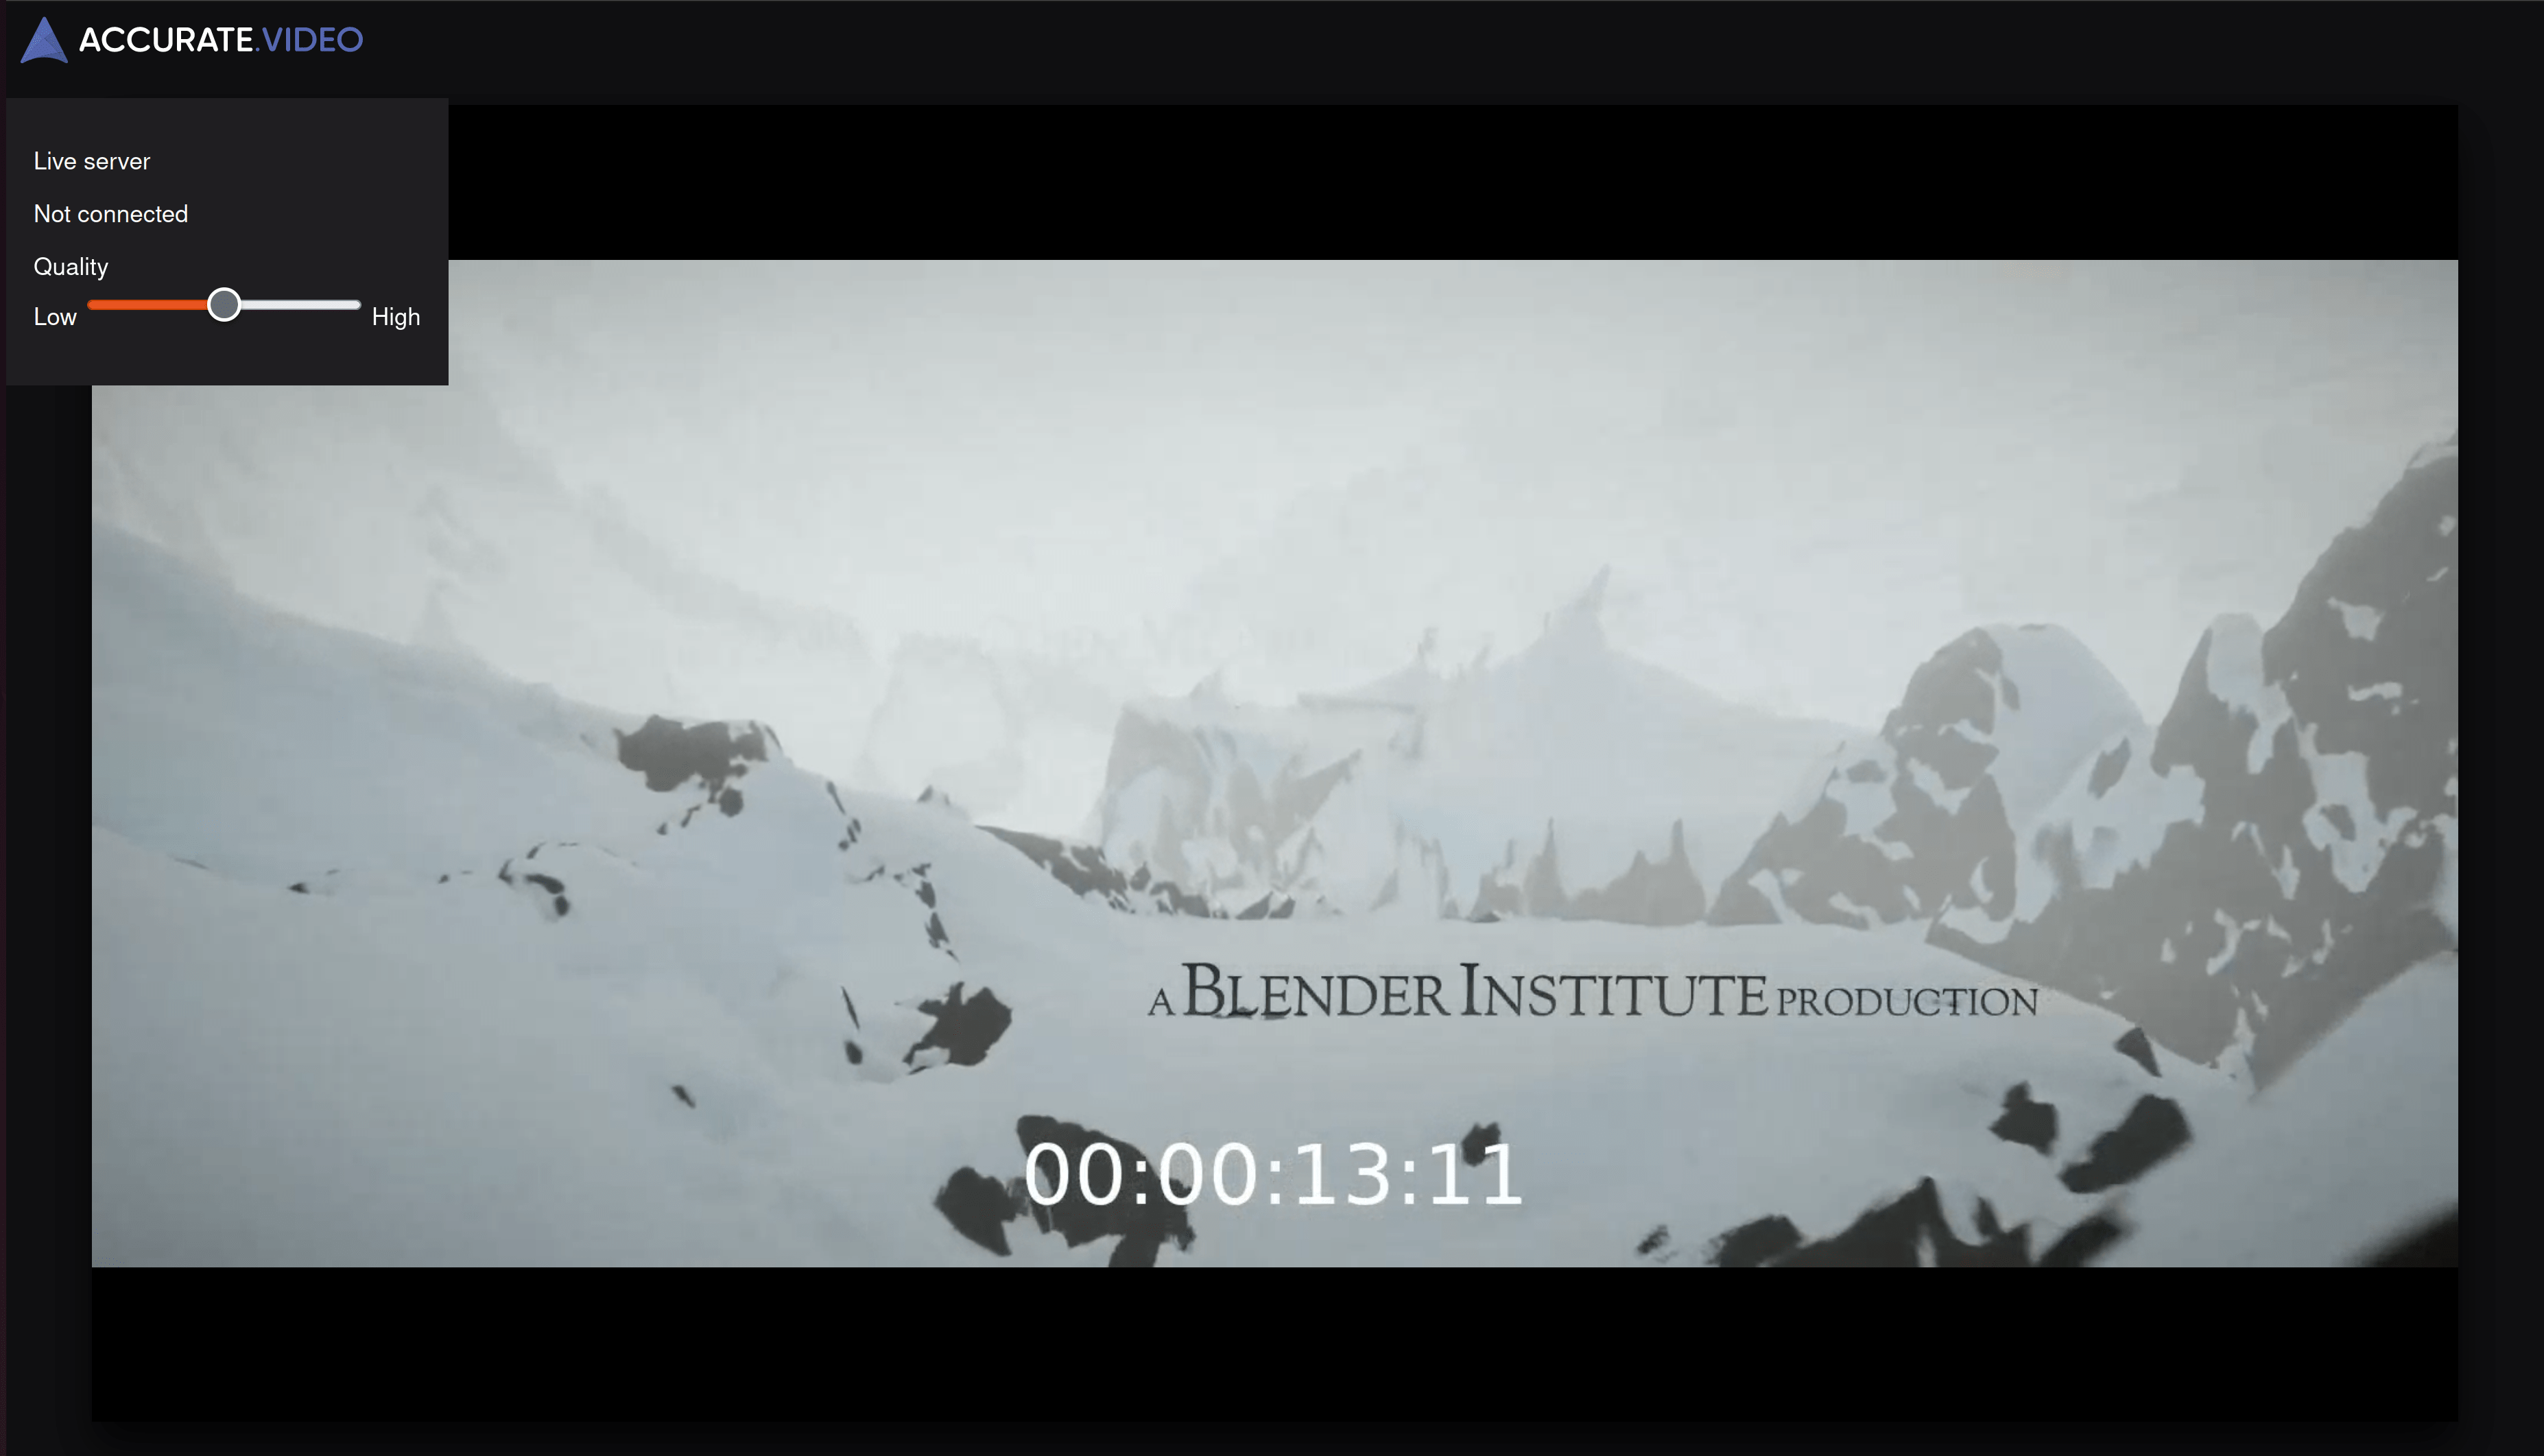
\includegraphics[width=0.32\textwidth]{AV3_before.png}
		%\cutpic{0.0cm}{0.3\textwidth}{AV2_before.png}
		%\cutpic{0.0cm}{0.3\textwidth}{AV3_before.png}
		\caption[Screenshots of the frontend.]{Screenshots of the Accurate Player when playing a video.}
		\label{figure:AV_before}
	\end{center}
\end{figure}
%
%
%
%
%
%
%
%
%
\sodef\spaceout{}{0pt plus 1fil}{.4em plus 1fil}{0pt}
%
In addition to this, the user interface of the Accurate Player has multiple control fields, which can be seen in Figure~\ref{figure:qualityslider}, \ref{figure:subtitles} and \ref{figure:othercontrols} and will be further described in the 
%
\begin{minipage}{0.5\textwidth}
%	
\vspace*{0.7em}
following.

	
Permanently fixed in the top left corner of the Accurate Player is a window that contains a slider to adjust the quality of the video in real time. This function does work for a video that is currently playing and for a frame of a video that is currently paused as well. This can be seen in Figure~\ref{figure:qualityslider}. 
In this project, the sliders for the RGB colour grading will be added in these windows, too. This is described in Section~\ref{subsection:implementation}.

\end{minipage}\begin{minipage}{0.05\textwidth}
	\ 
\end{minipage}\begin{minipage}{0.45\textwidth}
	
\begin{figure}[H]
	\begin{center}
		\cutpic{0.3cm}{0.9\textwidth}{qualityslider.png}
		\caption[Quality slider in the frontend.]{Quality slider in the frontend.}
		\label{figure:qualityslider} 
	\end{center}
\end{figure}
% \vfill
\end{minipage}

\vspace*{0.2em}
\makebox[\linewidth][l]{\spaceout{In the top right corner of the Accurate Player window that is displayed in the}}

\begin{minipage}{0.5\textwidth}
% \vspace*{0.7em}	
	\begin{figure}[H]
		\begin{center}
			\cutpic{0.3cm}{0.9\textwidth}{AV_settings.png}
			\caption[Subtitle and audio control field in the frontend.]{Subtitle and audio control field in the frontend.}
			\label{figure:subtitles}
		\end{center}
	\end{figure}
\vfill
\end{minipage}\begin{minipage}{0.05\textwidth}
	\ 
\end{minipage}\begin{minipage}{0.45\textwidth}
browser, two icons to expand further menus can be found. 
This includes a menu for subtitles and audio settings, which is divided into two parts for those settings. This control window can be seen in Figure~\ref{figure:subtitles}. It enables the audio functionalities for muting the audio or changing to a different audio track, which can be used for example if a video is available in different languages to switch between the languages. These options can be seen in Figure~\ref{figure:subtitles} on the right part of the control menu.
The left side of the window allows for enabling and disabling specific subtitles from a list of available subtitles. 
%
%
\end{minipage}

\begin{minipage}{0.45\textwidth}
	
Additionally, a menu with further settings can be found when expanding the menus. This menu can be seen in Figure~\ref{figure:othercontrols} and expands when clicking on the \textit{settings} symbol. Here, further settings, including the time format, the setting of keyboard shortcuts or the fading of the control options when playing the video can be adjusted. All of the above described menus for settings enhance the level of personalisation available to the user. The customisation options allow the 
%
%
\end{minipage}\begin{minipage}{0.05\textwidth}
	\ 
\end{minipage}\begin{minipage}{0.5\textwidth}
%
%
\begin{figure}[H]
	\begin{center}
		\cutpic{0.3cm}{0.9\textwidth}{AV_settings2.png}
		\caption[Window for settings in the frontend.]{Window for settings in the frontend.}
		\label{figure:othercontrols}
	\end{center}
\end{figure}
\vfill
\end{minipage}
%

% \vspace*{-0.2em}
user to adapt the Accurate Player to their preferences and expectations. 


With JIT techniques in the Accurate Player it is possible to play different formats in the browser without the transcoding into a browser friendly format.
This is possible, because the Accurate Player uses JIT techniques to dynamically handle the playback of different video formats on-the-fly, instead of relying on pre-transcoded video files. The video data is being processed in real-time, allowing for on-the-fly adjustment of options such as the quality slider or the RGB colour adjustment that is being implemented for this thesis project.









%-------------------------------------------------------------------------------------------------------
\subsection{JIT-WebRTC} \label{subsection:jit-webrtc}
% Describe the backend

The following description of the system's backend is based on the code base and the information from the \texttt{README} file~\cite{RM_Backend}.
JIT-WebRTC is a live transcoder with a WebRTC output. As described in Section~\ref{subsection_OverviewVideoStreamingComponents}, transcoding is the conversion of one digital data format into another~\cite{transcoding}.
The backend consists of three components: The MLT framework, \texttt{main.py} and a session service.


The user initiates a session through the browser, which then initiates the \texttt{main.py} script. The system's frontend that is displayed in the browser was described in Section~\ref{subsection:accuratevideo}.
Control commands are then sent from the browser to the Python backend with a WebRTC data channel.
From the \texttt{main.py} file, the control commands get sent to MLT via \texttt{stdout} (standard output) and \texttt{stdin} (standard input). These are the default input and output channels, that allow the Python script communication with other components.
Data written to \texttt{stdout} by the Python code can be captured or redirected and data from an external source can be read from \texttt{stdin} by the Python script~\cite{python}. The data flow of the control commands is highlighted in Figure~\ref{figure:controlcommands}.

\begin{figure}[H]
	\centering
	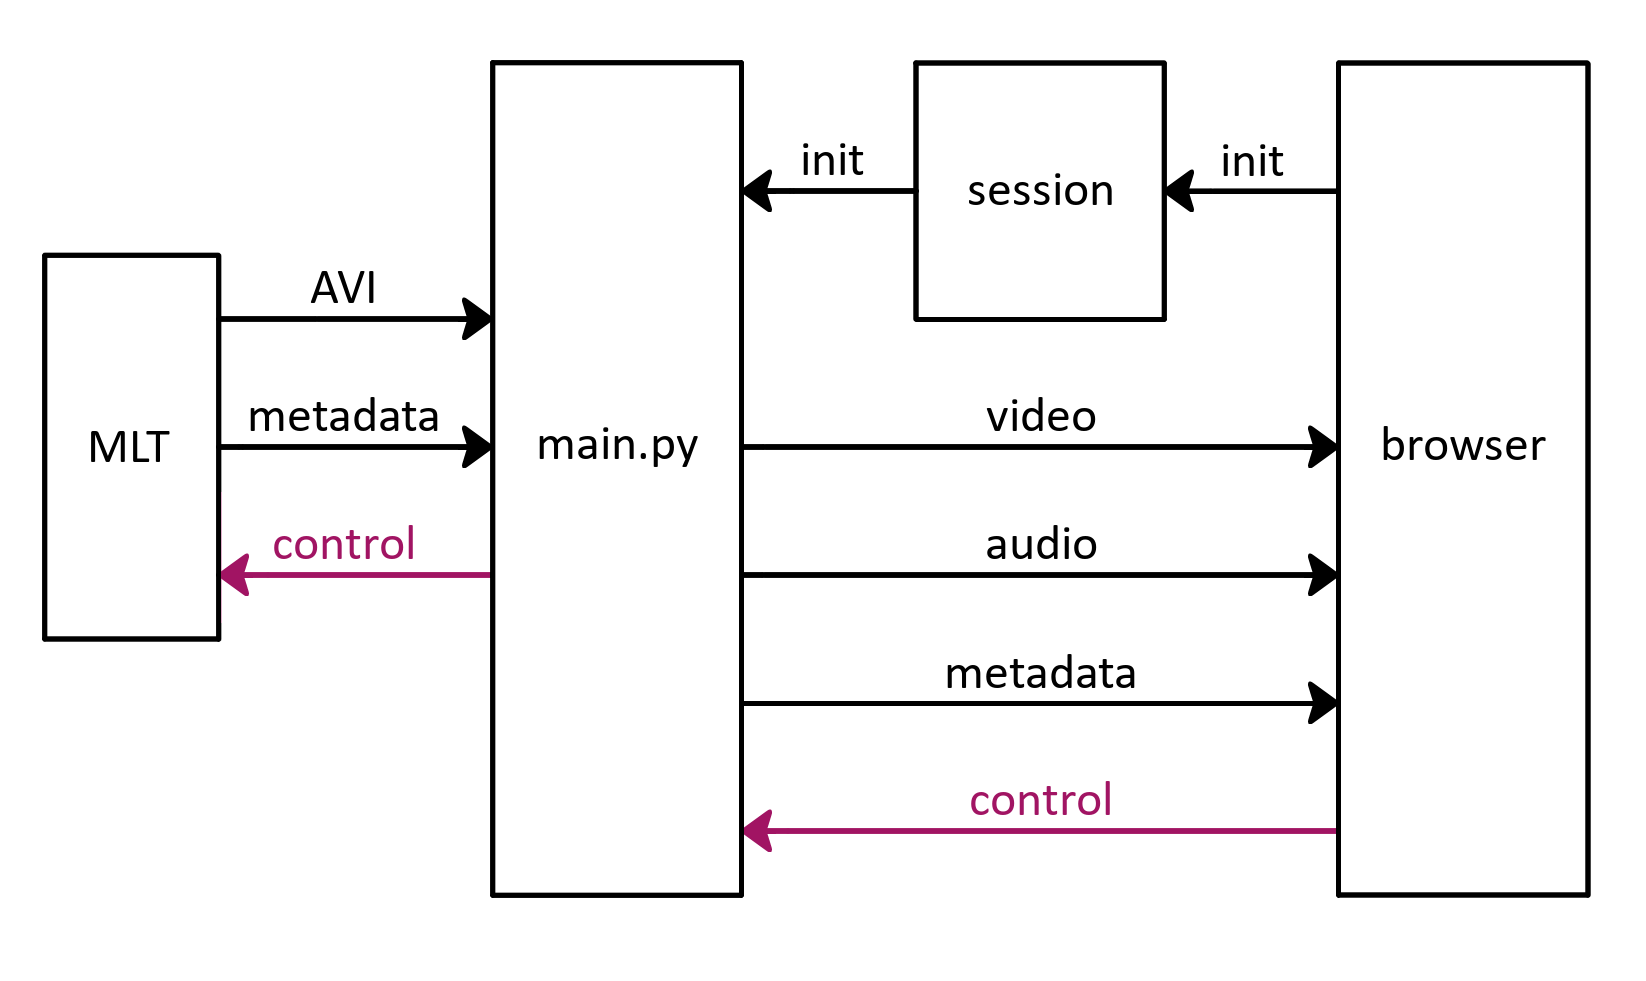
\includegraphics[width=0.5\textwidth]{IM_control.png}
	\caption{Control commands in the system architecture.}
	\label{figure:controlcommands}
\end{figure}


As a response, the MLT framework sends an AVI stream with the rendered video and audio, status messages and metadata to the Python backend. This is highlighted in Section~\ref{figure:avimetadata}.
AVI is a file format that can contain audio and video information to allow synchronised playback of audio and video components, as described in Section~\ref{subsection_OverviewVideoStreamingComponents}~\cite{avi}. 

\begin{figure}[H]
	\centering
	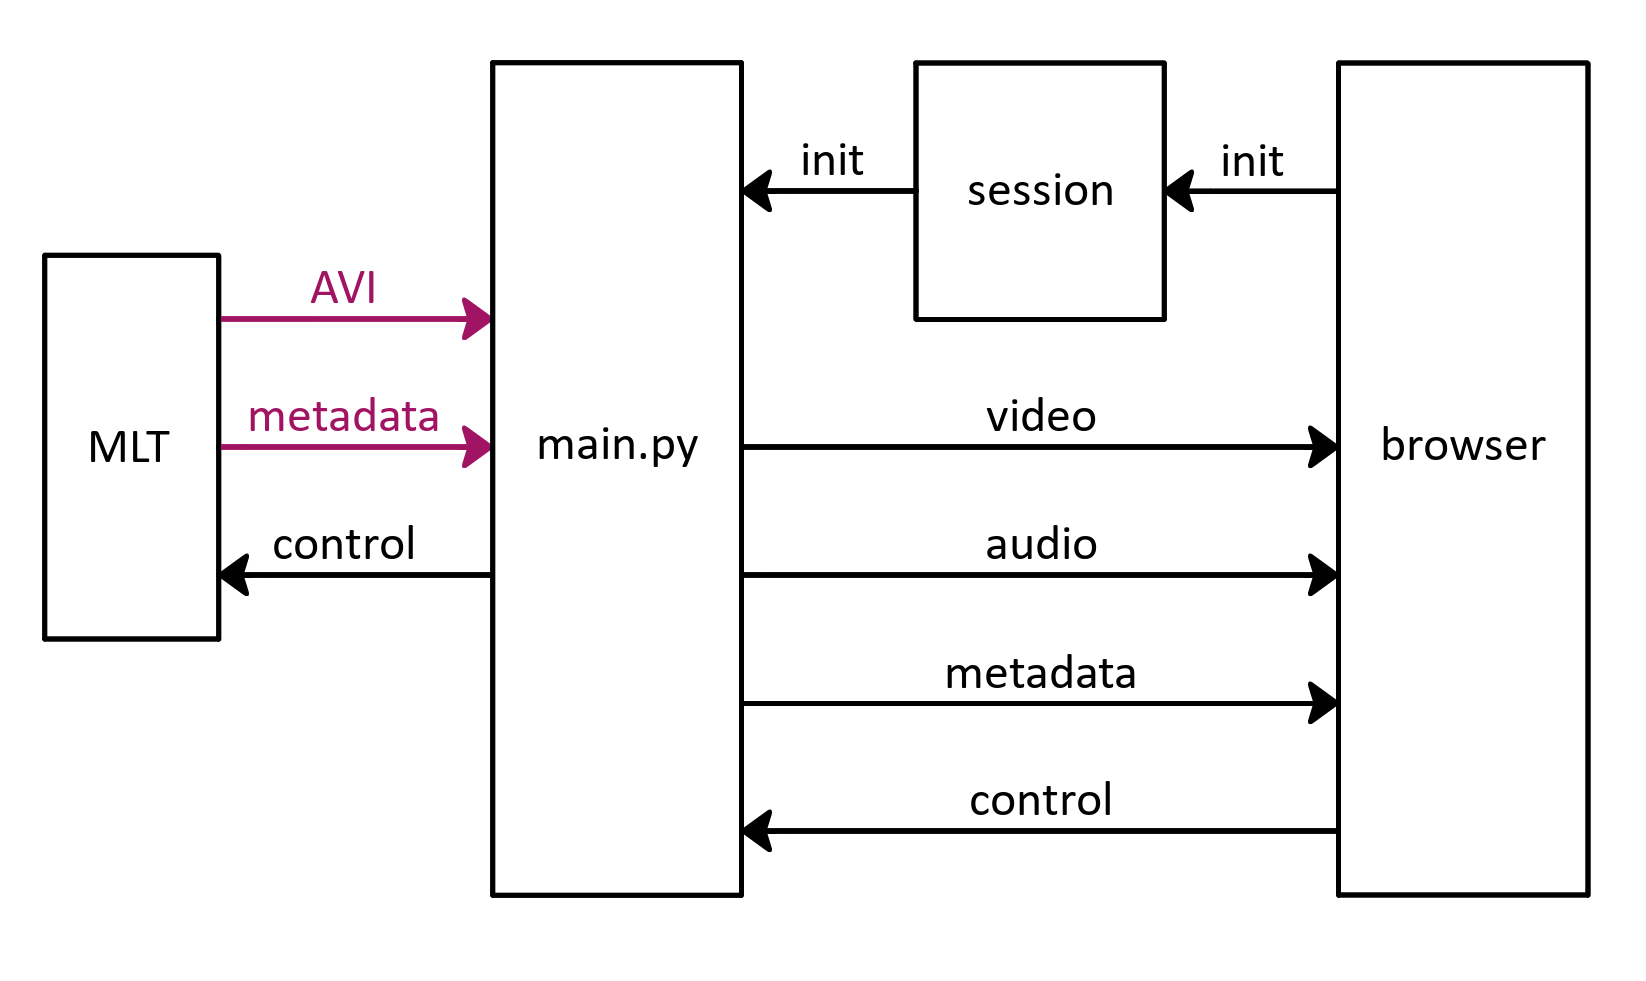
\includegraphics[width=0.5\textwidth]{IM_avi.png}
	\caption{AVI stream in the system architecture.}
	\label{figure:avimetadata}
\end{figure}


The audio and video from the incoming AVI stream is extracted by the \texttt{main.py} script to encode it for sending it to the browser with WebRTC. The WebRTC connection serves as a direct communication channel between the browser and the backend, enabling real-time data exchange, involving audio, video or other data streams. 


%It has the ability to extract specific channels from the rendered audio, to %be rendered to an stereo stream for WebRTC.
%It does not appear to be possible to encode surround sound for WebRTC, despite WebRTC using the Opus codec which is surround capable.
%This may be a limitation in `aiortc`, in WebRTC or in the browser, or all three.
%


The JavaScript client of the browser receives the video and audio to play it in the Accurate Player, which was described in Section~\ref{subsection:accuratevideo}. In addition to this, the browser
receives metadata from the \texttt{main.py} script and sends commands and responses over the control channel. This connection can be seen in Figure~\ref{figure:videoaudio}.


\begin{figure}[H]
	\centering
	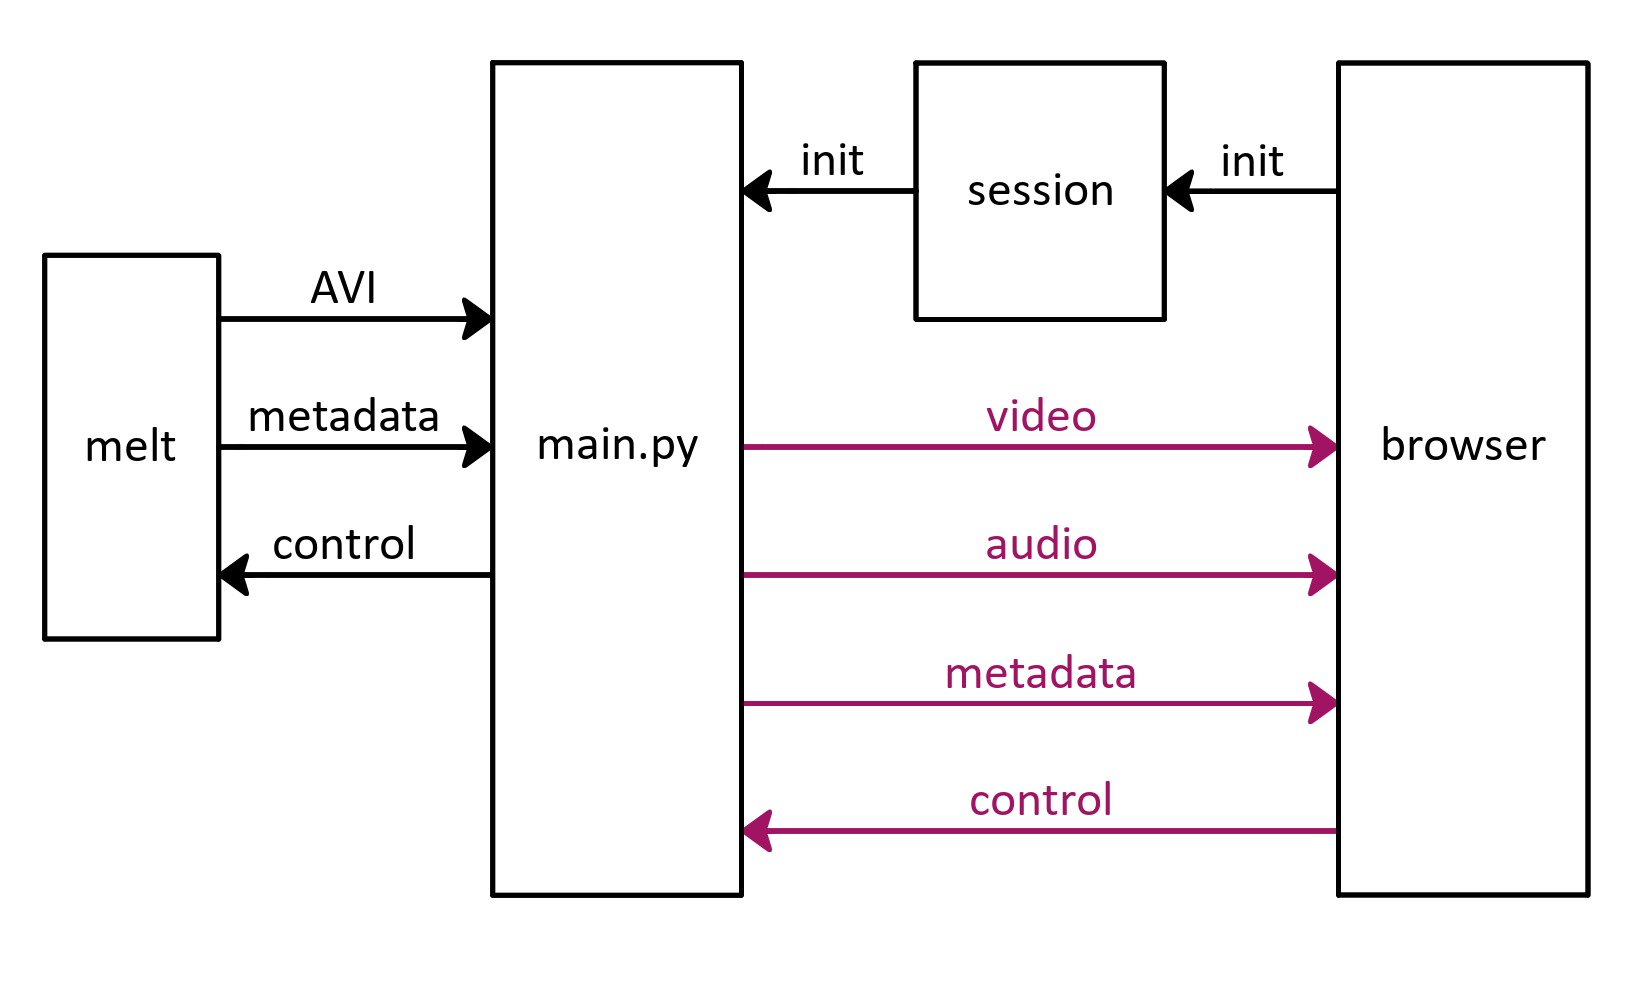
\includegraphics[width=0.5\textwidth]{IM_wrtc_control.png}
	\caption[WebRTC and control in the system architecture.]{WebRTC connection and control commands in the system architecture.}
	\label{figure:videoaudio}
\end{figure}

The MLT framework and the \texttt{main.py} script are started once for each JIT session.
The Java-based \texttt{Session} service is designed to support the machine-to-machine interaction between the browser and the Python backend. 
The \texttt{Session} service exposes a REST API (described in Section~\ref{subsection_OverviewVideoStreamingComponents}) for initiating a JIT session. 
%
% Additionally, it leverages AWS, specifically utilizing the Auto Scaling Group (ASG) feature to manage a cluster of instances dynamically, ensuring scalability and efficient distribution of JIT sessions across the instances in the cluster.
%
% AWS
%2. **AWS (Amazon Web Services):**
%- **Definition:** AWS is a cloud computing platform provided by Amazon. It offers a wide range of services, including computing power, storage, databases, machine learning, and more, allowing businesses to scale and grow without the need for significant upfront investments in physical infrastructure.
%
% ASG cluster
%3. **ASG Cluster (Auto Scaling Group):**
%- **Definition:** An Auto Scaling Group is an AWS service that automatically adjusts the number of compute instances (e.g., virtual machines) in response to changes in demand or other specified conditions. It helps ensure that the desired number of instances are available to handle varying workloads.
%
%
%
%`session` is a Java-based service that presents a REST api that can be used to start a new JIT session given a description of the media to use. It also has support for managing a full ASG cluster on AWS, and distribute new JIT sessions on the instances in 
%the ASG.
%
%For more information on each component see:
%* [`melt`](https://github.com/sirf/mlt.git)
%* [`main.py`](jit/README.md)
%* [`session`](session/README.md)
%
%
For development and testing without the session service, JIT can be started in a Docker container. This has been done for the implementation in this project.


%\begin{figure}[H]
%	\centering
%	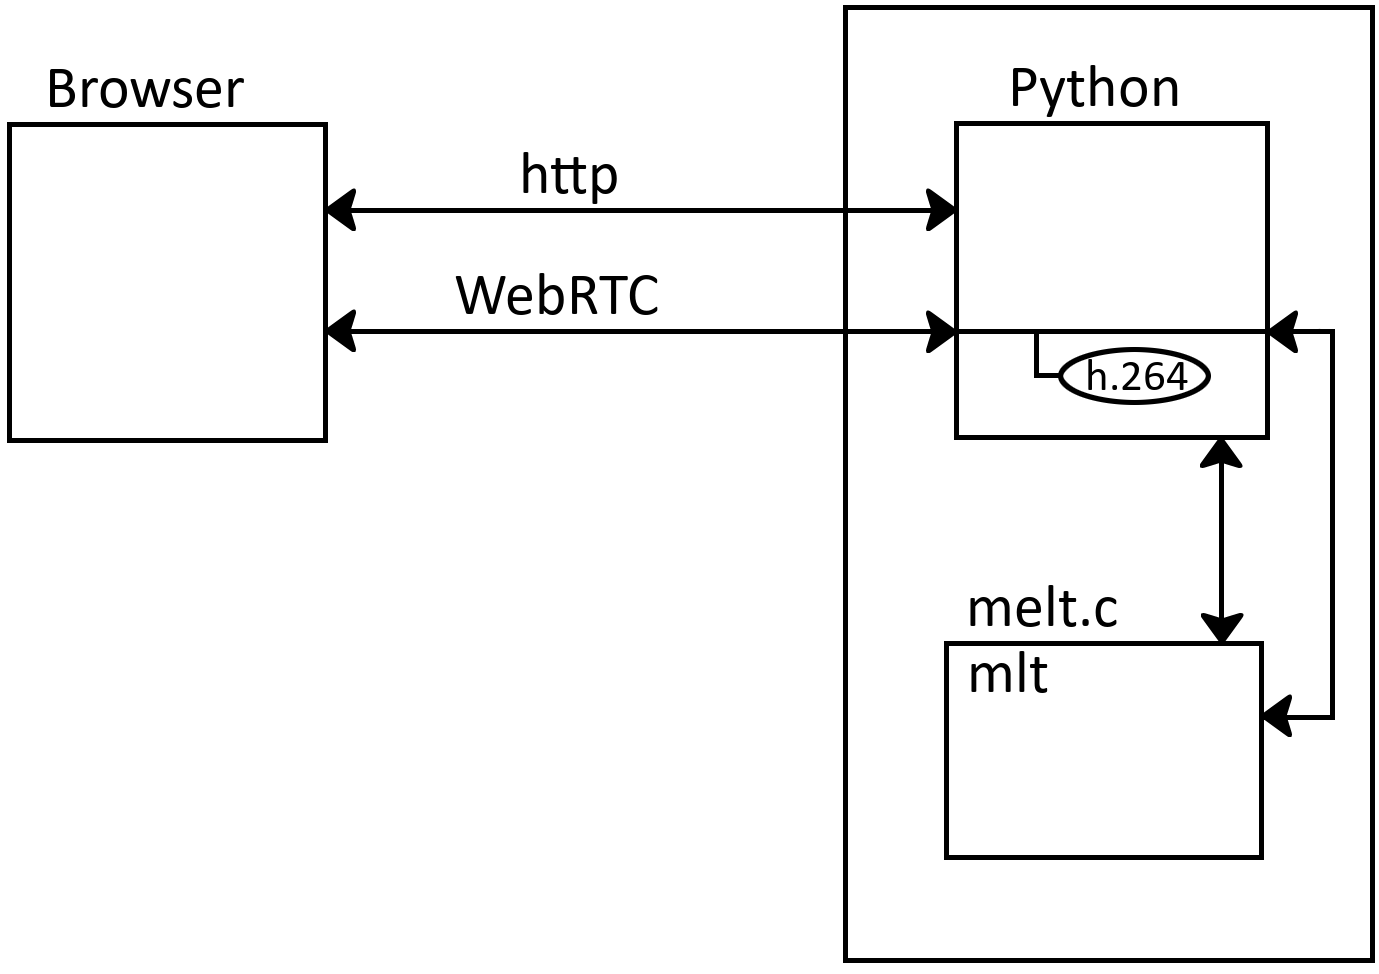
\includegraphics[width=0.6\textwidth]{IM2.png}
%	\caption{System architecture when run in a docker container.}
%\end{figure}


%## Development
%
%For development and quick testing without the session service, on can either start JIT as a docker, or run JIT directly on your computer. The latter has some problems if you're on an Apple ARM.
%
%Run the docker:
%
%`docker/main/main.sh --threads 16 --port 8080 $VIDEOFILE`
%
%Where `$VIDEOFILE` is either a local path or a URL. `threads` and `port` are both optional, with current default values set to 72 threads and port 8080.
%
%To run JIT directly, see [`jit/README.md`](jit/README.md).
%
%### Open Docker IPs
%
%Your Docker container will get an IP in the style of 172.17.0.\*. Using e.g. Docker CE on Linux this IP will be reachable from outside the container. However, on Docker Desktop for Mac, this IP will not be opened. This will cause problems. There is a service that can fix this. You **install and activate it once** by doing this:
%
%```
%# Install via Homebrew
%brew install chipmk/tap/docker-mac-net-connect
%
%# Run the service and register it to launch at boot
%sudo brew services start chipmk/tap/docker-mac-net-connect
%```
%
%
%## Deployment
%
%Currently the only way supported for deployment is by using EC2 instances on AWS. An AMI is created by CI on release, containing a 
%local instance of the `session-service`, together with `main.py`, `melt` and anything else needed to start JIT processes on the EC2 
%instance. For more information about what the AMI contains, and how configuration can be fed to it see [`ami/README.md`](ami/README.md).
%
%### Terraform
%
%Terraform modules are supplied that simplify setup of either single EC2 instances or a full ASG cluster of instances, including 
%`session-service` running as an orchestrator on ECS. See [`terraform/README.md`](terraform/README.md) for more information on 
%available modules, their parameters and outputs.
%





% \newpage
%-------------------------------------------------------------------------------------------------------
\subsection{MLT Filter Comparison} \label{subsection:meltfilter}



The goal for this thesis project is the on-the-fly adjustment of the RGB values of a video with sliders in the frontend. 
For this purpose, various MLT filters were examined and compared to identify the most suitable ones for implementing this functionality. 
RGB colour representation was described in Section~\ref{subsection:RGB} and the MLT framework was described in Section~\ref{subsection:melt}.

In Table~\ref{table:filter}, a selection of filters that influence the RGB representation of the video are listed. This includes the filter name, description and possible parameters that are listed on the MLT website~\cite{melt_filters}. Only parameters relevant to this thesis will be listed.
Then, those filters were applied to compare the visual results of applying them. 
The MLT filters \texttt{avfilter.colorbalance}, \texttt{avfilter\-.colorchannelmixer} and \texttt{frei0r\-.coloradj\_RGB} are selected for further analysis. They are listed with their description and parameters in Table~\ref{table:filter}, followed by a comparison of the visual results. Other MLT filters that change the visual appearance of the video can be seen in Appendix~\ref{appendix:differentMeltFilter}.



\begin{table}[H]
	\footnotesize
	\begin{tabular}{lp{4.4cm}p{4.5cm}}
		\toprule
		Name & Description & Parameters \\
		\midrule
		\texttt{avfilter.colorbalance} & Adjust the colour balance & 
		\tiny{
		\texttt{av.rs}: set red shadows \newline 
		\texttt{av.gs}: set green shadows \newline 
		\texttt{av.bs}: set blue shadows \newline 
		\texttt{av.rm}: set red midtones \newline 
		\texttt{av.gm}: set green midtones \newline 
		\texttt{av.bm}: set blue midtones \newline 
		\texttt{av.rh}: set red highlights \newline 
		\texttt{av.gh}: set green highlights \newline 
		\texttt{av.bh}: set blue highlights}
		\\
		\texttt{avfilter.colorchannelmixer} & Adjust colours by mixing colour channels & 
		\tiny{
		\texttt{av.rr}: set red gain for red channel \newline 
		\texttt{av.rg}: set green gain for red channel \newline 
		\texttt{av.rb}: set blue gain for red channel \newline 
		\texttt{av.ra}: set alpha gain for red channel \newline 
		\texttt{av.gr}: set red gain for green channel \newline 
		\texttt{av.gg}: set green gain for green channel \newline 
		\texttt{av.gb}: set blue gain for green channel \newline 
		\texttt{av.ga}: set alpha gain for green channel \newline 
		\texttt{av.br}: set red gain for blue channel \newline 
		\texttt{av.bg}: set green gain for blue channel \newline 
		\texttt{av.bb}: set blue gain for blue channel \newline 
		\texttt{av.ba}: set red gain for alpha channel \newline 
		\texttt{av.ar}: set red gain for alpha channel \newline 
		\texttt{av.ag}: set green gain for alpha channel \newline 
		\texttt{av.ab}: set blue gain for alpha channel \newline 
		\texttt{av.aa}: set alpha gain for alpha channel}
		\\
		\texttt{frei0r.coloradj\_RGB} & Simple colour adjustment & 
		\tiny{
		\texttt{R}: amount of red \newline 
		\texttt{G}: amount of green \newline 
		\texttt{B}: amount of blue}
		\\
		\bottomrule
	\end{tabular}
	\caption[List of MLT filters that influence the colour of a video.]{List of different MLT filters that influence the colour of a video with their name, description and parameters.}
	\label{table:filter}
\end{table}



%Execution of \texttt{melt https://s3.eu-central-1.amazonaws.com/accurate-player\--demo-assets/timecode/sintel-2048-timecode-stereo.mp4 \\ -filter avfilter.colorbalance av.rs=1 av.gm=1 av.bh=1}:


%\begin{minipage}{0.5\textwidth}
%	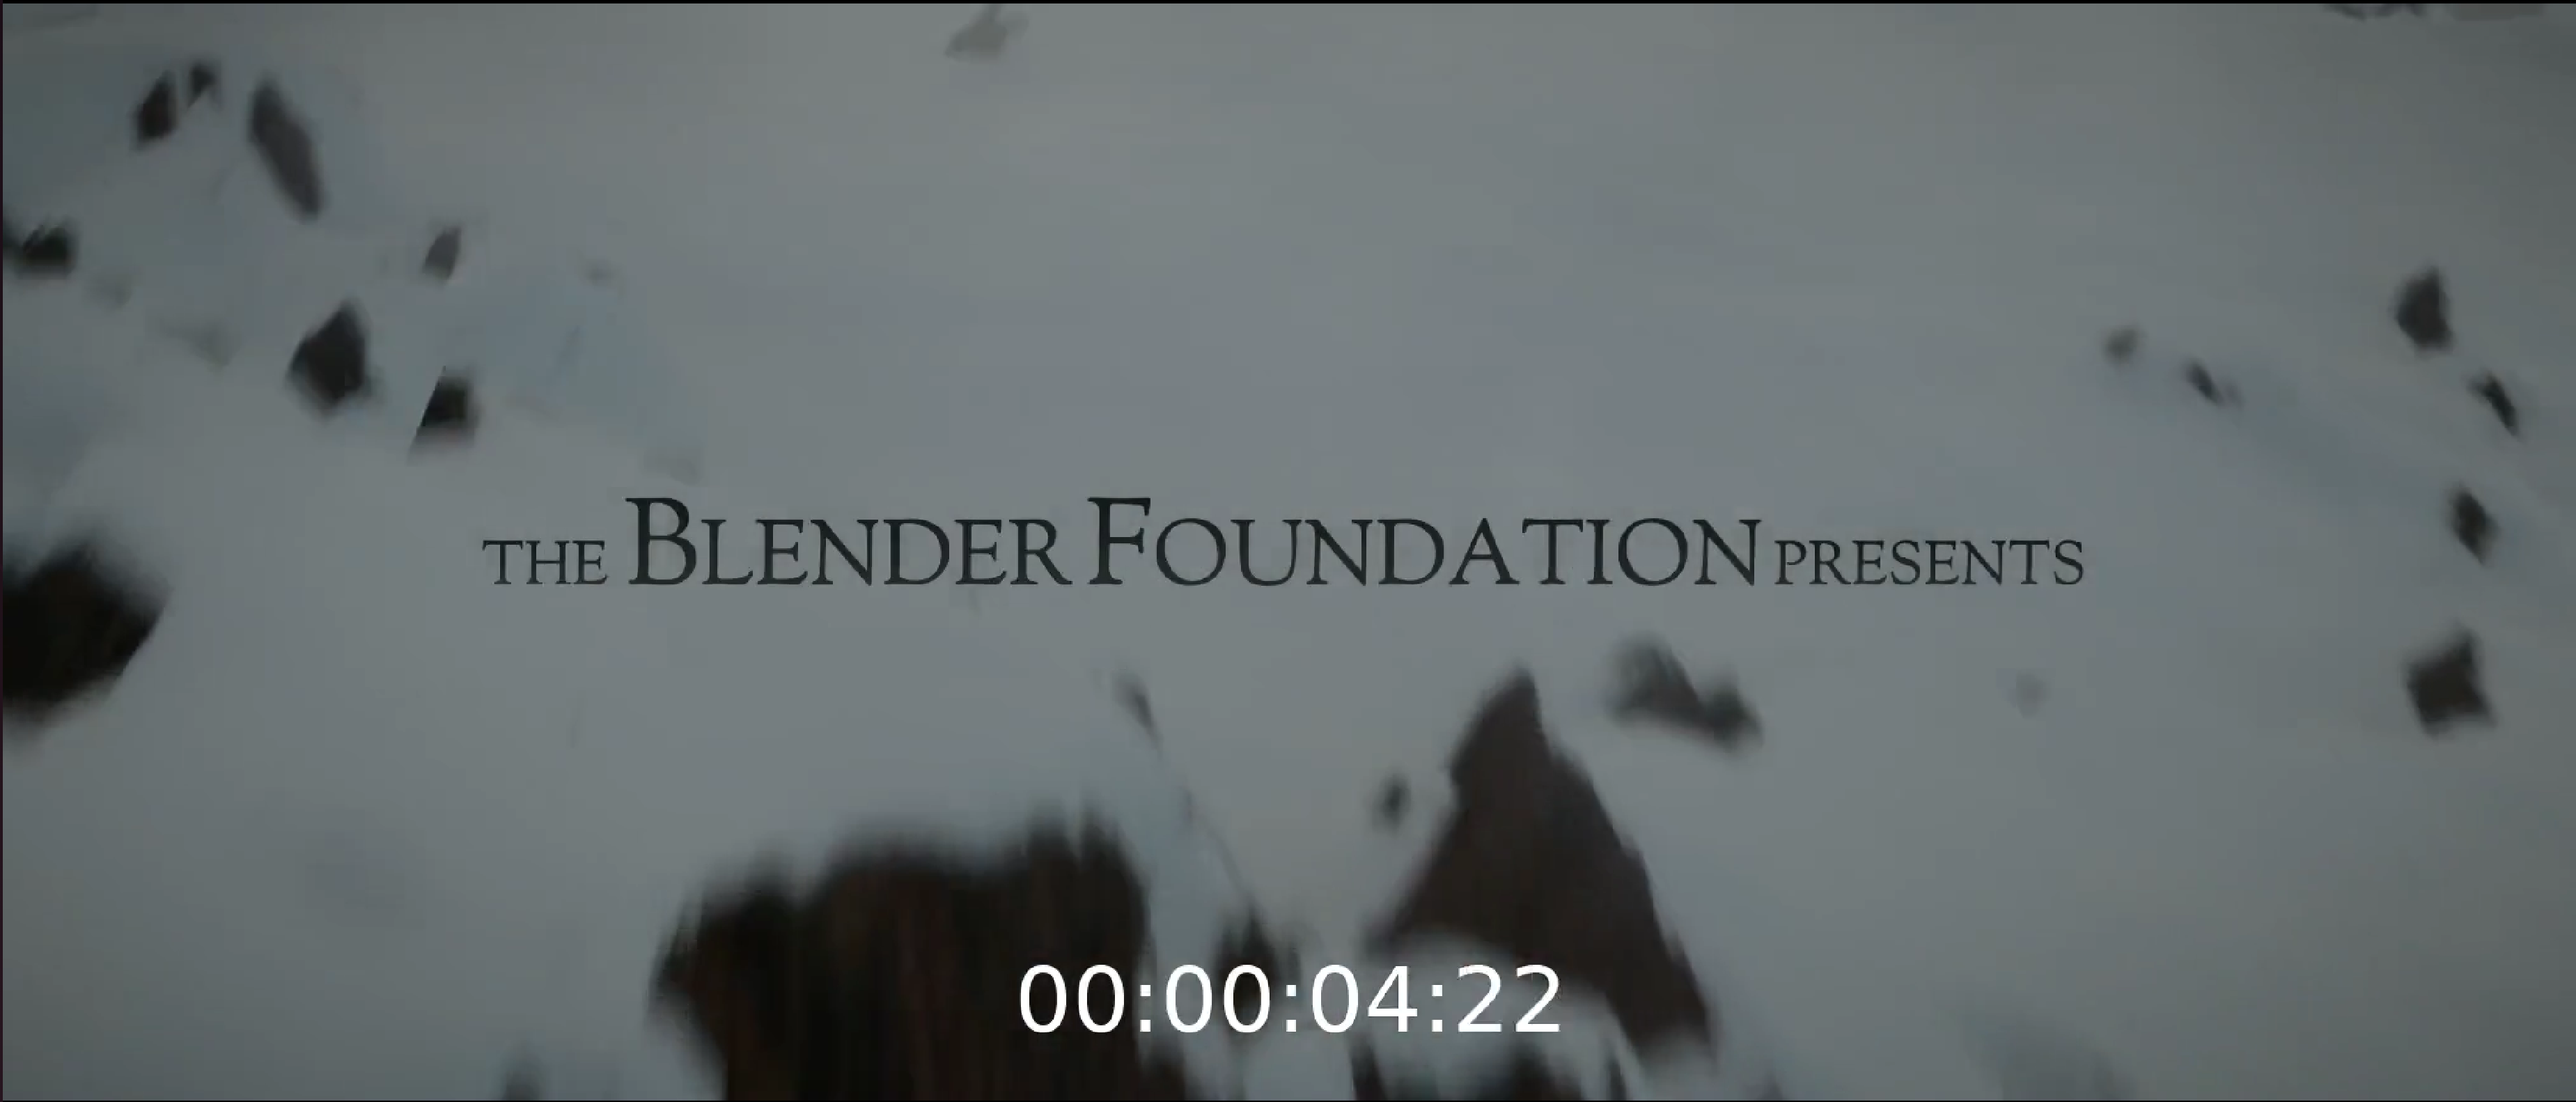
\includegraphics[width=0.9\textwidth]{colourdefault.png}
%	Original colours
%\end{minipage}\begin{minipage}{0.5\textwidth}
%	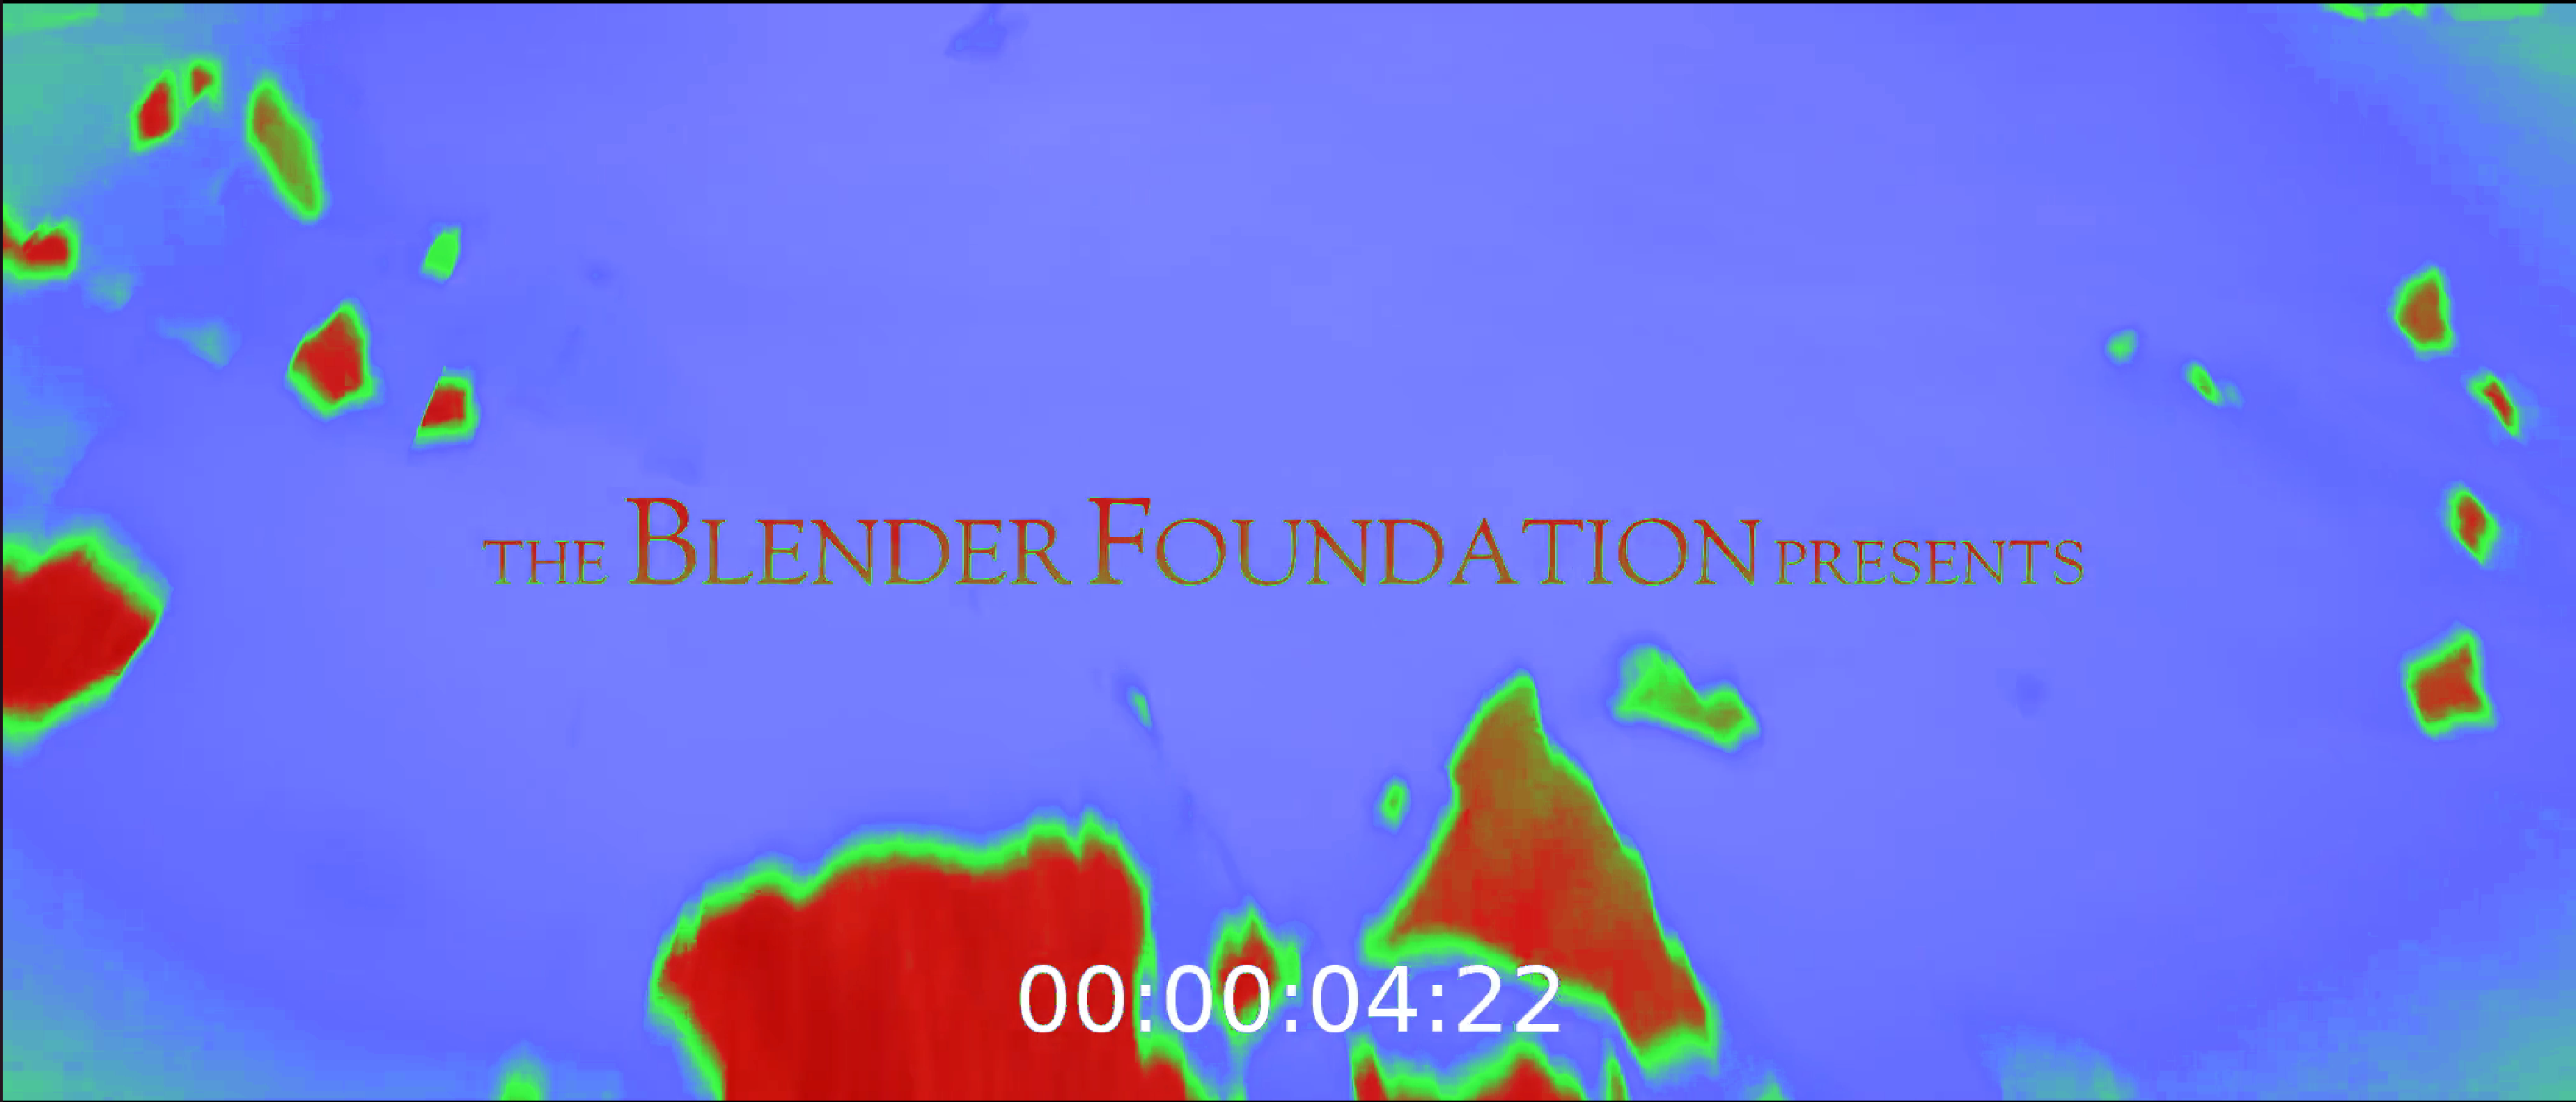
\includegraphics[width=0.9\textwidth]{colourhigh.png}
%	Colours with \texttt{av.rs=1} \texttt{av.gm=1} \texttt{av.bh=1}
%\end{minipage}

%Adding filter to \texttt{local\_melt.py} to execute it in the Accurate Player using JIT:
%`
%\begin{center}
%	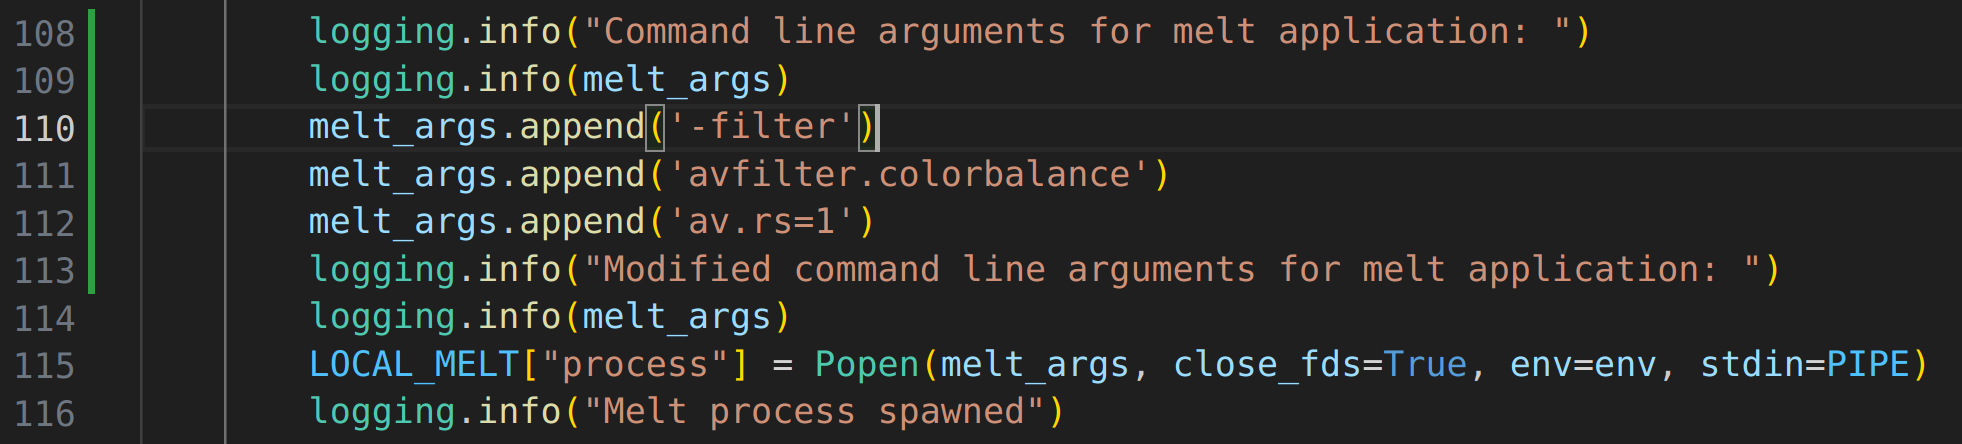
\includegraphics[height=0.13\textwidth]{code.png}
%	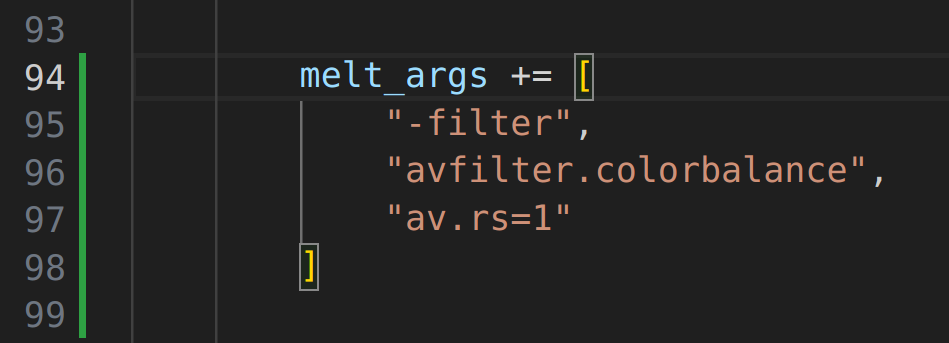
\includegraphics[height=0.13\textwidth]{codecleaner.png}
%\end{center}
%
%\begin{center}
%	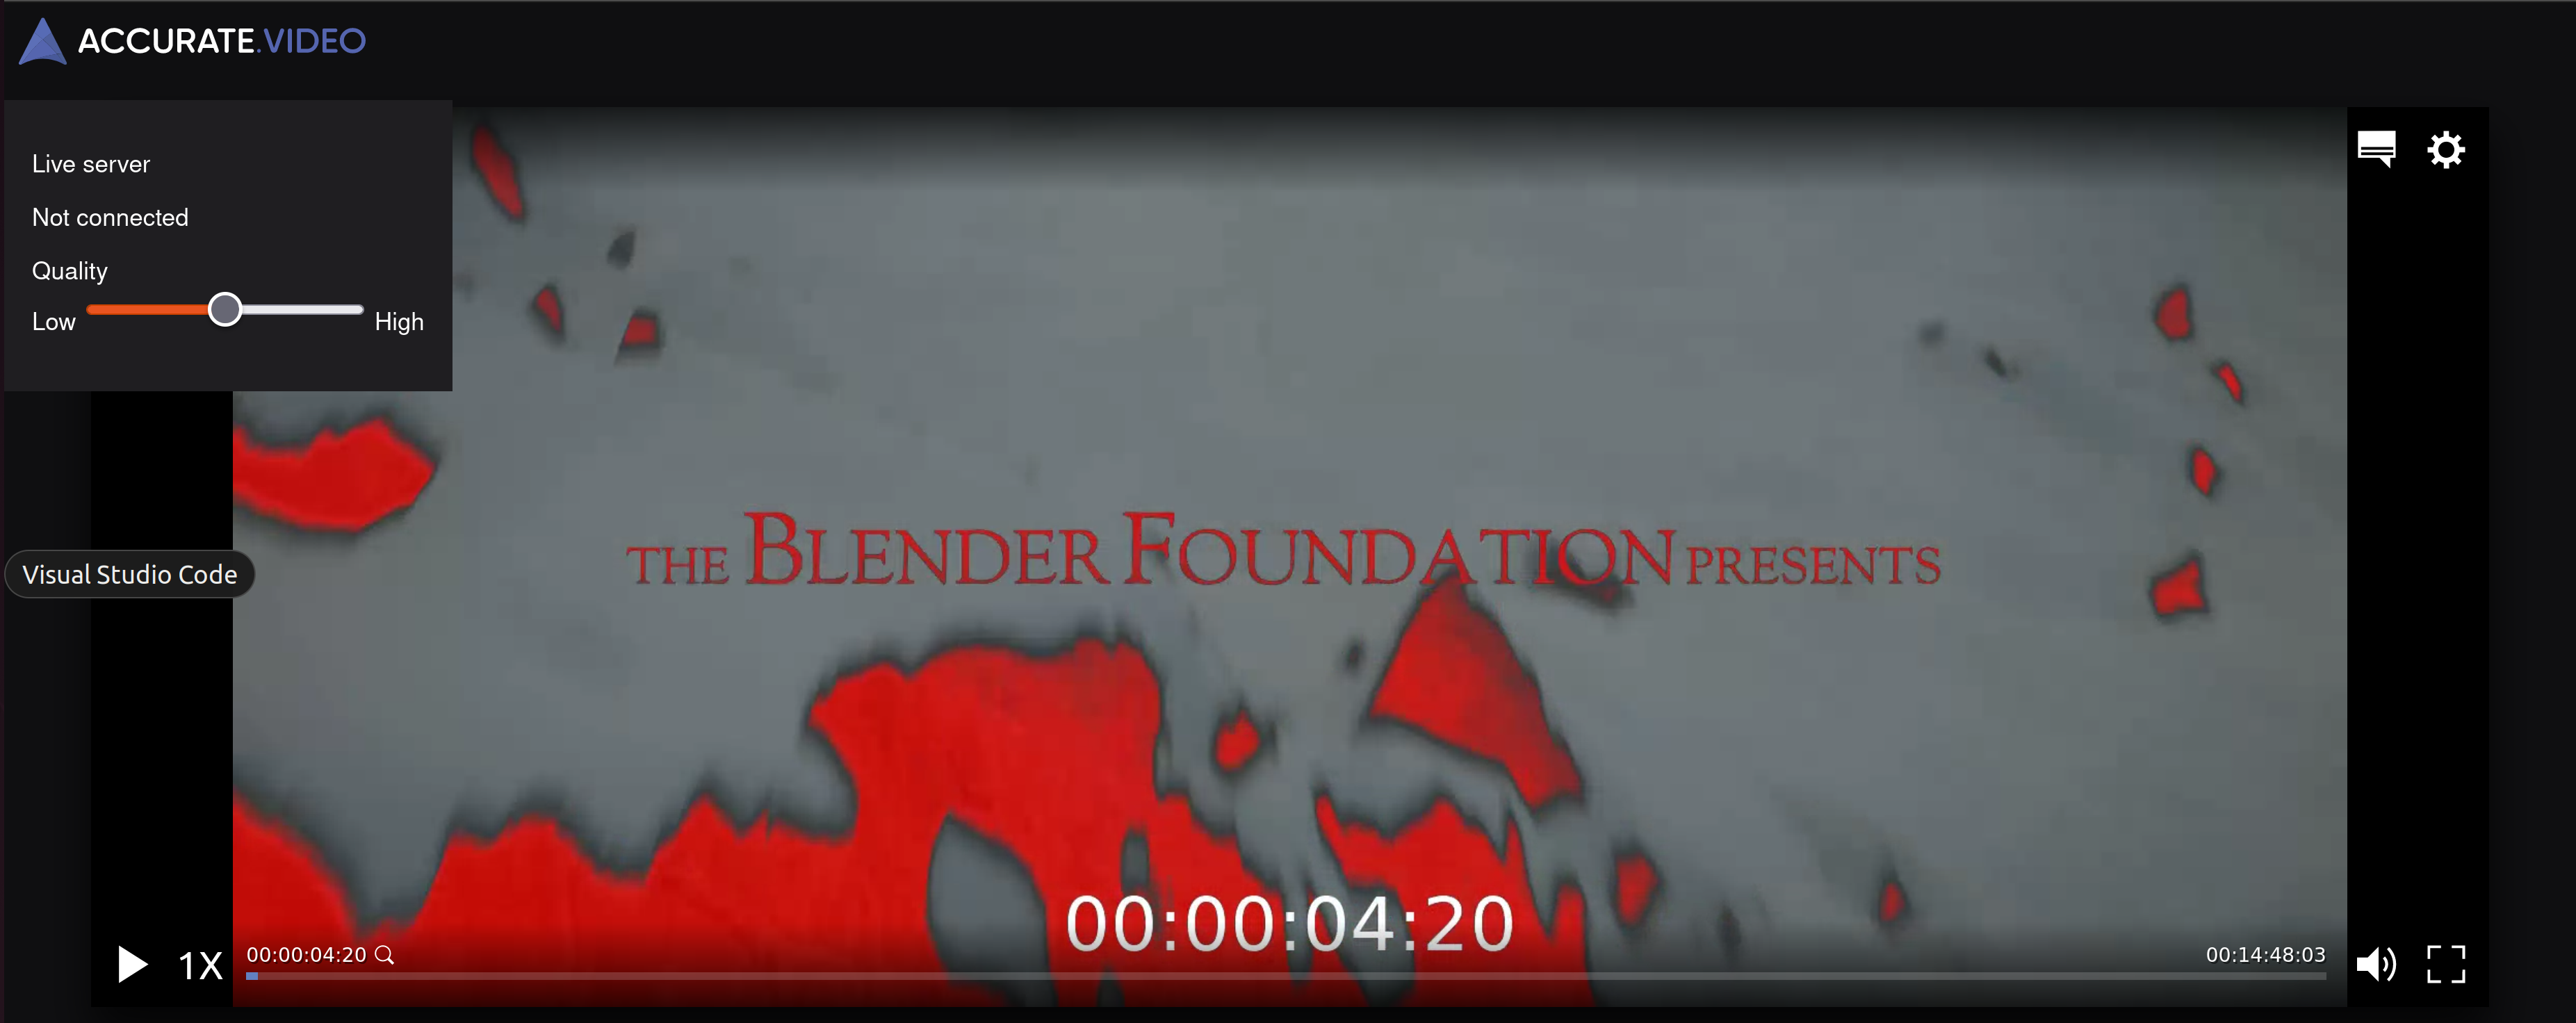
\includegraphics[width=0.8\textwidth]{ap_red.png}
%\end{center}


To introduce the listed filters and their parameters, the maximum value to adjust the red tones of the video will be tested and described. 
%
In addition to this, it needs to be tested, if multiple parameters of the same filter can be applied simultaneously. For this evaluation, the filters with their different parameters for green and red are applied to the same frame of the test video file. Regarding the RGB colour model, this should result in a yellow toned output frame. The functionality of the RGB colour model was explained in Section~\ref{subsection:RGB}. 
%
In the following comparison, the adjustment of all three colour channels (red, green and blue) will be presented.

For the purpose of evaluating and comparing, two frames were selected from the example video file of the short film \textit{Sintel}. Each of those frames has a distinct colour scheme. One frame shows a snow landscape and the \textit{Blender Institute Production} text, while the other frame shows an elderly man in a warm lighted indoor setting. The original frames $343$ and $3377$ can be seen in Figure~\ref{figure:nofilter} for reference.


\begin{figure}[H]
	\begin{center}
		\cutpic{0.3cm}{0.45\textwidth}{nofilter_snow.png}
		\cutpic{0.3cm}{0.45\textwidth}{nofilter_man.png}
		\caption[Frames $343$ and $3377$ from the test video file without a filter.]{Frames $343$ on the left and $3377$ on the right, extracted from the test video file \textit{Sintel} without a filter.}
		\label{figure:nofilter}
	\end{center}
\end{figure}



%The filters were applied with the locally installed version of the Melt framework with the following CLI command and test video file:
%\begin{lstlisting}[language=bash, numbers=none]
%	melt -filter <filter_name> <filter_parameter> https://s3.eu-central-1.amazonaws.com/accurate-player-demo-assets/timecode/sintel-2048-timecode-stereo.mp4 -consumer xgl
%\end{lstlisting}


In the following, the filter application and parameters of each filter are introduced and described with the example of the adjustment of the colour red.














%--------------------------------------------------------------------------------------
\subsubsection*{Filter \texttt{avfilter.colorbalance}}

The parameters of the filter \texttt{avfilter.colorbalance} take input values as a floats between $-1$ and $1$. The filter has individual parameters to set the shadows, midtones and highlights per colour (red, green and blue). The results of the different parameters set on the maximum value of $1$ for adjusting the red shadows with \texttt{av.rs=1}, the red midtones with \texttt{av.rm=1} and the red highlights with \texttt{av.rg=1} can be seen in Figure~\ref{figure:rs1rm1rh1}.

\begin{figure}[H]
	\begin{center}
		\cutpic{0.32cm}{0.3\textwidth}{rs_snow.png}
		%\hspace*{0.01\textwidth}
		\cutpic{0.32cm}{0.3\textwidth}{rm_snow.png}
		%\hspace*{0.01\textwidth}
		\cutpic{0.32cm}{0.3\textwidth}{rh_snow.png}
		% \small{
		%\texttt{av.rs=1} \hspace*{0.22\textwidth} \texttt{av.rm=1} \hspace*{0.23\textwidth} \texttt{av.rh=1}}
		\cutpic{0.32cm}{0.3\textwidth}{rs_man.png}
		%\hspace*{0.01\textwidth}
		\cutpic{0.32cm}{0.3\textwidth}{rm_man.jpg}
		%\hspace*{0.01\textwidth}
		\cutpic{0.32cm}{0.3\textwidth}{rh_man.png}
		\small{
		\texttt{av.rs=1} \hspace*{0.22\textwidth} \texttt{av.rm=1} \hspace*{0.23\textwidth} \texttt{av.rh=1}}
		\caption[Different parameters from the filter \texttt{avfilter.colorbalance} applied.]{Different parameters from the filter \texttt{avfilter.colorbalance} applied: Left with \texttt{av.rs=1} for red shadows, middle with \texttt{av.rm=1} for red midtones and right with \texttt{av.rh=1} for red highlights.}
			\label{figure:rs1rm1rh1}
	\end{center}
\end{figure}

To achieve an even colouring result of the frame, which would be applicable for a colour change with one slider per colour, the parameters for the shadows, midtones and highlights can be adjusted simultaneously when adjusting one colour. In Figure~\ref{figure:rsrmrh1}, the shadows, midtones and highlights for the red value are set to $1$. 

\begin{figure}[H]
	\begin{center}
		\cutpic{0.3cm}{0.45\textwidth}{rsrmrh_snow.png}
		\cutpic{0.3cm}{0.45\textwidth}{rsrmrh_man.png}
		\caption[Parameters set to $1$ for red using the \texttt{avfilter.colorbalance} filter.]{All parameters for the adjustment of the red tones with the value $1$ from the filter \texttt{avfilter.colorbalance} applied: \texttt{av.rs=1}, \texttt{av.rm=1} and \texttt{av.rh=1}.}
		\label{figure:rsrmrh1}
	\end{center}
\end{figure}

To assess the effects of the combined colour adjustment of multiple colours, the values for green and red (shadows, midtones and highlights) are set to the maximum of $1$ and applied simultaneously. The parameters that are applied for this evaluation are \texttt{av.rs=1}, \texttt{av.rm=1}, \texttt{av.rh=1}, \texttt{av.gs=1}, \texttt{av.gm=1} and \texttt{av.gh=1}.
This results in yellow toned pictures, that can be seen in Figure~\ref{figure:cb_yellow}.


\begin{figure}[H]
	\begin{center}
		\cutpic{0.3cm}{0.45\textwidth}{cb_yellow.png}
		\cutpic{0.3cm}{0.45\textwidth}{cb_yellow_man.png}
		\caption[Red and green parameters set to $1$ with \texttt{avfilter.colorbalance}.]{All parameters for red and green with the value $1$ from the filter \texttt{avfilter.colorbalance} applied: \texttt{av.rs=1}, \texttt{av.rm=1}, \texttt{av.rh=1}, \texttt{av.gs=1}, \texttt{av.gm=1} and \texttt{av.gh=1}.}
		\label{figure:cb_yellow}
	\end{center}
\end{figure}













%--------------------------------------------------------------------------------------

\subsubsection*{Filter \texttt{avfilter.colorchannelmixer}}

The parameters of the filter \texttt{avfilter.colorchannelmixer} take input values as floats between $-2$ and $2$. The filter has individual parameters to set the red, green, blue or alpha gain for the red, green, blue or alpha channel. The application of the maximum value of 2 for the red gain on the red channel, alpha gain on the red channel and red gain on the alpha channel can be seen in Figure~\ref{figure:rrraar}.

\begin{figure}[H]
	\begin{center}
		\cutpic{0.32cm}{0.3\textwidth}{rr_snow.png}
		%\hspace*{0.01\textwidth}
		\cutpic{0.32cm}{0.3\textwidth}{ra_snow.png}
		%\hspace*{0.01\textwidth}
		\cutpic{0.32cm}{0.3\textwidth}{ar_snow.png}
		% \small{
			%\texttt{av.rs=1} \hspace*{0.22\textwidth} \texttt{av.rm=1} \hspace*{0.23\textwidth} \texttt{av.rh=1}}
		\cutpic{0.32cm}{0.3\textwidth}{rr_man.png}
		%\hspace*{0.01\textwidth}
		\cutpic{0.32cm}{0.3\textwidth}{ra_man.png}
		%\hspace*{0.01\textwidth}
		\cutpic{0.32cm}{0.3\textwidth}{ar_man.png}
		\small{
			\texttt{av.rr=2} \hspace*{0.22\textwidth} \texttt{av.ra=2} \hspace*{0.23\textwidth} \texttt{av.ar=2}}
		\caption[Different parameters from \texttt{avfilter.colorchannelmixer} applied.]{Different parameters from the filter \texttt{avfilter.colorchannelmixer} applied: Left with \texttt{av.rr=2} for red gain on the red channel, middle with \texttt{av.ra=2} for alpha gain on the red channel and right with \texttt{av.ar=2} for red gain on the alpha channel.}
		\label{figure:rrraar}
	\end{center}
\end{figure}


Additionally, in Figure~\ref{figure:rrbrgr}, the red gain on the red, blue and green channel is applied simultaneously. The parameter settings for this are \texttt{av.rr=2}, \texttt{av.gr=2} and \texttt{av.br=2}.


\begin{figure}[H]
	\begin{center}
		\cutpic{0.3cm}{0.45\textwidth}{rrbrgr_snow.png}
		\cutpic{0.3cm}{0.45\textwidth}{rrbrgr_man.png}
		\caption[Red gain set to $2$ with \texttt{avfilter.colorchannelmixer}.]{Red gain with the value $2$ for the red, green and blue channel from the filter \texttt{avfilter.colorchannelmixer} applied: \texttt{av.rr=2}, \texttt{av.gr=2} and \texttt{av.br=2}.}
		\label{figure:rrbrgr}
	\end{center}
\end{figure}

To assess the effects of the combined colour adjustment of multiple colours for the \texttt{avfilter.colorchannelmixer} filter, the values for the green gain on the green channel and the red gain on the red channel are set to the maximum of $2$ and applied simultaneously. 
The parameters that are applied are \texttt{av.rr=2} and \texttt{av.gg=2}.
This results in yellow toned pictures, that can be seen in Figure~\ref{figure:rrgg}.


\begin{figure}[H]
	\begin{center}
		\cutpic{0.3cm}{0.45\textwidth}{rrgg_snow.png}
		\cutpic{0.3cm}{0.45\textwidth}{rrgg_man.png}
		\caption[Red and green gain set to $2$ with \texttt{avfilter.colorchannelmixer}.]{Red gain on red channel and green gain on green channel with the value $2$ from the filter \texttt{avfilter.colorchannelmixer} applied: \texttt{av.rr=2} and \texttt{av.gg=2}.}
		\label{figure:rrgg}
	\end{center}
\end{figure}







%--------------------------------------------------------------------------------------
\subsubsection*{Filter \texttt{frei0r.coloradj\_RGB}}

The parameters of the filter \texttt{frei0r.coloradj\_RGB} take input values as floats between $0$ and $1$. The filter has individual parameters to set the red, green, blue value for RGB adjustment. The application of the red parameter with the maximum value of $1$ can be seen in Figure~\ref{figure:r}.


\begin{figure}[H]
	\begin{center}
		\cutpic{0.3cm}{0.45\textwidth}{r_snow.png}
		\cutpic{0.3cm}{0.45\textwidth}{r_man.png}
		\caption[Red parameter set to $1$ with \texttt{frei0r.coloradj\_RGB}.]{Red parameter with the value $1$ from the filter \texttt{frei0r.coloradj\_RGB} applied: \texttt{R=1}.}
		\label{figure:r}
	\end{center}
\end{figure}

To assess the effects of the combined colour adjustment of multiple colours for the \texttt{frei0r.coloradj\_RGB} filter, the values for the green and red parameter are set to the maximum value $1$ and applied simultaneously. The applied parameters are \texttt{R=1} and \texttt{G=1}. This results in yellow toned pictures, which can be seen in Figure~\ref{figure:rg}.


\begin{figure}[H]
	\begin{center}
		\cutpic{0.3cm}{0.45\textwidth}{rg_snow.png}
		\cutpic{0.3cm}{0.45\textwidth}{rg_man.png}
		\caption[Red and green parameter set to $1$ with \texttt{frei0r.coloradj\_RGB}.]{Red and green parameter with the value $1$ from the filter \texttt{frei0r.coloradj\_RGB} applied: \texttt{R=1} and \texttt{G=1}.}
		\label{figure:rg}
	\end{center}
\end{figure}




\subsubsection*{Evaluation}

%the filters are compared regarding the result of the application of one flter and for this the vibrance and intensity is the important factor and regarding the mixing of colours and here vibrance and intensity are the important aspects as well



The MLT filters \texttt{avfilter.colorbalance}, \texttt{avfilter\-.colorchannelmixer} and \texttt{frei\-0r\-.coloradj\_RGB} are compared regarding the colour vibrance and intensity of the result. This analysis of the filters above was conducted regarding the colour red in depth and a side-by-side comparison can be seen in Figure~\ref{figure:redcomp}. The colour changes of green and blue work analogically and are displayed in Figure~\ref{figure:filtersG} and \ref{figure:filtersB}.
% For the comparison of the result of the single colour filter application, the following parameters per filter are chosen:
%
%The results of the change of a single colour (red, green and blue) for each of the filters can be seen as a side-by-side comparison:

\begin{figure}[H]
	\centering
	\begin{tabular}{c|c|c}
		
		\footnotesize{\texttt{avfilter.colorbalance}} & \footnotesize{\texttt{avfilter.colorchannelmixer}} & \footnotesize{\texttt{frei0r.coloradj\_RGB}} \\
		
		\scriptsize{\texttt{av.rs=1} \texttt{av.rm=1} \texttt{av.rh=1}} & \scriptsize{\texttt{av.rr=2}} & \scriptsize{\texttt{R=1}} \\
		
		\cutpic{0.3cm}{0.29\textwidth}{rsrmrh_snow.png} & \cutpic{0.3cm}{0.29\textwidth}{rr_snow.png} & \cutpic{0.3cm}{0.29\textwidth}{r_snow.png} \\
		
		\cutpic{0.3cm}{0.29\textwidth}{rsrmrh_man.png} & \cutpic{0.3cm}{0.29\textwidth}{rr_man.png} & \cutpic{0.3cm}{0.29\textwidth}{r_man.png} \\
		
	\end{tabular}
	
	\caption{Comparison of red filter option of all three filters.}
	\label{figure:redcomp}
	
\end{figure}


\begin{figure}[H]
	\centering
	\begin{tabular}{c|c|c}
		
		\footnotesize{\texttt{avfilter.colorbalance}} & \footnotesize{\texttt{avfilter.colorchannelmixer}} & \footnotesize{\texttt{frei0r.coloradj\_RGB}} \\
		
		\scriptsize{\texttt{av.gs=1} \texttt{av.gm=1} \texttt{av.gh=1}} & \scriptsize{\texttt{av.gg=2}} & \scriptsize{\texttt{G=1}} \\
		
		\cutpic{0.3cm}{0.29\textwidth}{gsgmgh_snow.png} & \cutpic{0.3cm}{0.29\textwidth}{gg_snow.png} & \cutpic{0.3cm}{0.29\textwidth}{g_snow.png} \\
		
		\cutpic{0.3cm}{0.29\textwidth}{gsgmgh_man.png} & \cutpic{0.3cm}{0.29\textwidth}{gg_man.png} & \cutpic{0.3cm}{0.29\textwidth}{g_man.png} \\
		
	\end{tabular}
	
	\caption{Comparison of green filter option of all three filters.}
	\label{figure:filtersG}
	
\end{figure}


\begin{figure}[H]
	\centering
	\begin{tabular}{c|c|c}
		
		\footnotesize{\texttt{avfilter.colorbalance}} & \footnotesize{\texttt{avfilter.colorchannelmixer}} & \footnotesize{\texttt{frei0r.coloradj\_RGB}} \\
		
		\scriptsize{\texttt{av.bs=1} \texttt{av.bm=1} \texttt{av.bh=1}} & \scriptsize{\texttt{av.bb=2}} & \scriptsize{\texttt{B=1}} \\
		
		\cutpic{0.3cm}{0.29\textwidth}{bsbmbh_snow.png} & \cutpic{0.3cm}{0.29\textwidth}{bb_snow.png} & \cutpic{0.3cm}{0.29\textwidth}{b_snow.png} \\
		
		\cutpic{0.3cm}{0.29\textwidth}{bsbmbh_man.png} & \cutpic{0.3cm}{0.29\textwidth}{b_man.png} & \cutpic{0.3cm}{0.29\textwidth}{b_man.png} \\
		
	\end{tabular}
	
	\caption{Comparison of blue filter option of all three filters.}
	\label{figure:filtersB}
	
\end{figure}




In the Figures above, it can be seen that the red, green and blue tones of the frames with the filter \texttt{avfilter.colorbalance} applied is the most intense and vibrant. This makes the filter \texttt{avfilter.colorbalance} a suitable choice regarding the adjustment of a single colour channel, because a broader range in the colour intensity leads to more options for personalisation.



In Figure~\ref{figure:yellowcomp}, the results of the application of two mixed colours for each of the filters can be seen as a side-by-side comparison. The chosen colours are red and green, which leads to a yellow result.

\begin{figure}[H]
	\centering
	\begin{tabular}{c|c|c}
		
		\footnotesize{\texttt{avfilter.colorbalance}} & \footnotesize{\texttt{avfilter.colorchannelmixer}} & \footnotesize{\texttt{frei0r.coloradj\_RGB}} \\
		
		\scriptsize{\texttt{av.rs=1} \texttt{av.rm=1} \texttt{av.rh=1}} & \scriptsize{\texttt{av.rr=2}} & \scriptsize{\texttt{R=1}} \\
		\scriptsize{\texttt{av.gs=1} \texttt{av.gm=1} \texttt{av.gh=1}} & \scriptsize{\texttt{av.gg=2}} & \scriptsize{\texttt{G=1}} \\
		
		\cutpic{0.3cm}{0.29\textwidth}{cb_yellow.png} & \cutpic{0.3cm}{0.29\textwidth}{rrgg_snow.png} & \cutpic{0.3cm}{0.29\textwidth}{rg_snow.png} \\
		
		\cutpic{0.3cm}{0.29\textwidth}{cb_yellow_man.png} & \cutpic{0.3cm}{0.29\textwidth}{rrgg_man.png} & \cutpic{0.3cm}{0.29\textwidth}{rg_man.png} \\
		
	\end{tabular}
	
	\caption{Comparison of red filter option of all three filters.}
	\label{figure:yellowcomp}
	
\end{figure}

It can be seen, that the colour of the \texttt{avfilter.colorbalance} is the most intense and vibrant again, which confirms the results of the previous comparison regarding the single colour adjustment of red, green and blue. This makes the filter \texttt{avfilter.colorbalance} a suitable choice for the implementation of the RGB colour adjustment with sliders in the frontend, because it leads to a broader colour range and more options for personalisation. The filter \texttt{avfilter.colorbalance} shows the most intense colour results for single colour adjustments as well as for mixed colours.

In the above presented tests, which are visualised in the middle in Figure~\ref{figure:redcomp}, \ref{figure:filtersG}, \ref{figure:filtersB} and \ref{figure:yellowcomp}, the results of the \texttt{avfilter.colorchannelmixer} filter appear to have more depth and look more dynamic, because the colour gain was only executed on the respective colour channels. This can be an aspect, that lets the user achieve more aesthetically pleasing results but the overall intensity of the colours is lower. In addition to this, the expected behaviour of sliders for RGB colour adjustment might not be to only change the colour intensity on one of the respective colour channel. Based on this, the filter \texttt{avfilter.colorbalance} seems to deliver the most fitting results in those criteria.


The results of the filter \texttt{frei0r.coloradj\_RGB}, that can be seen on the right in Figure~\ref{figure:redcomp}, \ref{figure:filtersG}, \ref{figure:filtersB} and \ref{figure:yellowcomp} seem to have darker and less vibrant results, that do not present the expected colours as accurately as the other two filters. This does not make it a fitting choice for the RGB adjustment with sliders.


In conclusion, the \texttt{avfilter.colorbalance} filter leads to the most vibrant and intense results of the above listed selection of filters. Additionally it has the option to adapt the shadows, midtones and highlights individually, which creates the option for more pre-adjustments of the results in the backend or for introducing more sliders or options for the user-sided adjustment as future work.
But on the downside, to tone the whole frame evenly, three instead of one parameter have to be changed and applied -- for the shadows, midtones and highlights for each colour slider.
When applying this with and without JIT, no performance difference was noticeable but for an accurate evaluation of this, performance tests would have to be performed and the implementations of the filters would need to be examined, which exceeds the scope of this project.
%
A deeper examination and evaluation of the different options of other MLT filters is an interesting option for future work or for Codemill to implement. For this thesis project, the filter \texttt{avfilter.colorbalance} will be used, because its results look the most vibrant and fitting for the expected outcome of RGB colour adjustment.

In Figure~\ref{figure:septopus}, the seven basic colour combinations of the subtractive colour model can be seen with the application of the filter \texttt{avfilter.colorbalance}. For this, the RGB values were set to either $1.0$ or $0$, which are the maximum and default values of this filter. 



\begin{figure}[H]
	\begin{center}
		\cutpic{0.3cm}{0.8\textwidth}{septopus.png}
		\caption[Basic colours with the application of the filter \texttt{avfilter.colorbalance}.]{Basic colours of the subtractive colour model with the application of the filter \texttt{avfilter.colorbalance}.}
		\label{figure:septopus}
	\end{center}
\end{figure}

For comparison, the original frame 3447 from the test video file can be seen in Figure~\ref{figure:septo_nofilter} without applied filters.

\begin{figure}[H]
	\begin{center}
		\cutpic{0.3cm}{0.4\textwidth}{septopus_nofilter.png}
		\caption[Frame 3447 of the test video file without a filter.]{Frame 3447 of the test video file without a filter.}
		\label{figure:septo_nofilter}
	\end{center}
\end{figure}












% \newpage
%-------------------------------------------------------------------------------------------------------
\subsection{Implementation} \label{subsection:implementation}
% Discuss the technologies and tools chosen for the implementation.

In this Section, the implementation is described. This is separated into three parts, that are described individually: The frontend, the protocol buffer and the application of the filter in the backend. For the implementation, the sliders for each colour (red, green and blue) are added in the frontend. The input value of those sliders are sent with a protocol buffer to the backend, where the values are used to set the parameters of the MLT filter \texttt{avfilter.colorbalance} before applying the filter. This results in the user-sided RGB adjustment of the video colouring, which is played back in the frontend.

%-----------------------------------------------------------------------------------------------------------
\subsubsection*{Frontend}
%
\vspace*{-0em}
\begin{minipage}{0.52\textwidth}
In the frontend, input sliders for the user-sided adjustment of the RGB values are added below the already existing slider for the quality adjustment. This is located in the overlay windows in the top left corner. The sliders are coloured according to their associated functions in red, green and blue. This can be seen in Figure~\ref{figure:sliders}.

The HTML code for the red slider can be seen below. The other sliders for green and blue work analogically. The input range is set between $-100$ and $100$, to divide it later by $100$ to achieve a float value between $-1$ and 




\end{minipage}\begin{minipage}{0.04\textwidth}
\ 
\end{minipage}\begin{minipage}{0.44\textwidth}
\begin{figure}[H]
	\begin{center}
		\cutpic{0.3cm}{0.9\textwidth}{sliders.png}
		\caption[Sliders for RGB colour adjustment.]{Sliders for RGB colour adjustment.}
		\label{figure:sliders}
	\end{center}
\end{figure}
\hfill
\end{minipage}

\vspace*{-1em}
$1$ for the filter parameter. The default value is set to $0$. The input value from the slider then gets read out in a TypeScript file. 


\begin{lstlisting}[language=html, numbers=none]
	<p>
		<label for="red-slider">Red</label><br />
		Low
		<input
			type="range"
			min="-100"
			max="100"
			value="0"
			class="slider"
			id="red-slider"
		/>
		High
	</p>
\end{lstlisting}

The design of the sliders is defined in a CSS file: The \texttt{class} attribute of the slider uses the design setting of the pre-existing quality slider and the \texttt{id} with the value \texttt{red-slider} sets the background colour of the slider to red. 










%-----------------------------------------------------------------------------------------------------------
\subsubsection*{Protocol Buffer}

For the data transfer between frontend and backend for the colour grading, fields and enums are added to the \texttt{.proto} file. Protocol buffers are explained in Section~\ref{subsection:protocolbuffer}. The 
%
\begin{minipage}{0.54\textwidth}
\vspace*{-0.2em}
\begin{lstlisting}[style=protobufStyle, numbers=none]
syntax = "proto2";
	
message JitControl {
	...
	optional float red_value = 4; 
	optional float green_value = 5; 
	optional float blue_value = 6; 
}
	
enum ControlType {
	...
	RED_VALUE = 7;
	GREEN_VALUE = 8;
	BLUE_VALUE = 9;
}
\end{lstlisting}
\hfill
\end{minipage}\begin{minipage}{0.04\textwidth}
	\ 
\end{minipage}\begin{minipage}{0.42\textwidth}
\vspace*{0.6em}
values that are retrieved by the previously described sliders for the RGB value are transferred with this data structure.
In the code, the message \texttt{JitControl} and the enum \texttt{ControlType} can be seen. 
In the message, three optional fields for the red, green and blue value are defined as \texttt{red\_value}, \texttt{green\_value} and \texttt{blue\_value} to represent the RGB colour values. 
In the enum, the three constants (\texttt{RED\_VALUE}, \texttt{GREEN\_VALUE} and \texttt{BLUE\_VALUE}) are added. 
Through the sliders in the frontend, users can manipulate these values for red, green

\end{minipage}

and blue. The input values of those sliders are read out and assigned to the enum \texttt{JITAction} in the frontend. They are then transmitted to the backend with the proto2 data format. The application of the MLT filters with the retrieved values is described in the following part.











%-----------------------------------------------------------------------------------------------------------
\subsubsection*{Application of the MLT filter}


\begin{minipage}{0.60\textwidth}
	The application of the MLT filter is implemented in the \texttt{jit.c} file. To be able to apply multiple values for the three different colour channels at once, the command needs to be sent to MLT with all of the 
\end{minipage}\begin{minipage}{0.04\textwidth}
	\ 
\end{minipage}\begin{minipage}{0.36\textwidth}
	{\tiny\begin{lstlisting}[language=c, numbers=none]
		float red_value;
		float green_value;
		float blue_value; \end{lstlisting}}
	\vfill
\end{minipage}
\vspace*{0.1em}

according parameters set, else the other parameters will be overwritten with the default value $0$. This refers to the achieving of mixed colour results, including for example yellow, which can be created by adjusting the red and the green colour channel. The previous values for each colour channel need to be sent to the backend together with the changed value to prevent the overwriting of the already adjusted colours with the default value. This is implemented with initialising global variables for each of the colours that are set to the current value in each call. This can be seen in the code snippet above.

The application of the MLT filter with the current input values from the sliders is implemented in the function \texttt{jit\_action()}, that has a MLT producer as a parameter. In the code below, the beginning of the function can be seen. The MLT properties, consumer and producer are retrieved and set. Then the filter \texttt{avfilter.colorbalance} is set. The comparison of the different filter options can be seen in Section~\ref{subsection:meltfilter}.


\begin{lstlisting}[language=c, numbers=none, columns=fullflexible]	
mlt_properties properties = MLT_PRODUCER_PROPERTIES(producer);
mlt_consumer consumer = mlt_properties_get_data(properties, "transport_consumer", NULL);
...	
mlt_producer service = mlt_producer_service(producer);
mlt_filter filter = mlt_factory_filter(service, "avfilter.colorbalance", NULL);	
\end{lstlisting}


In the following code excerpt, a pointer \texttt{jit\_control} is declared, which casts a value into the type \texttt{JitControl}.
Then, a switch statement is started, based on the value of \texttt{jit\_control}.
The \texttt{->} operator is used to access the type field of the \texttt{jit\_control} structure and depending on the value, the execution will jump to the corresponding case within the switch statement.

\begin{lstlisting}[language=c, numbers=none, columns=fullflexible]		
JitControl *const jit_control = (JitControl*) value;
switch (jit_control->type) { ...
\end{lstlisting}

Three cases are implemented: One for each colour value (red, green, blue). In the following, the switch case for the adjustment of the red value is explained in more detail. The other cases work analogically.

In the code part below, the case for the red value can be seen. First, the red value that is retrieved from the slider in the frontend is assigned to the variable \texttt{red\_value}. Then, an \texttt{mlt\_properties} object is created for setting the filter parameters later on. 

\begin{lstlisting}[language=c, numbers=none, columns=fullflexible]			
case CONTROL_TYPE__RED_VALUE:
	red_value = jit_control->red_value;
	{
		mlt_properties filter_props_red = mlt_filter_properties(filter);
\end{lstlisting}

In the first if statement of this case, the red value is added to the filter properties. For this, the value needs to be in the input range of the filter parameter, which has to be a float between $-1$ and $1$. Then, a string containing the value is created, because the function \texttt{mlt\_properties\_set} requires the value for the filter parameter in String format. After this, the filter properties are set to this value. Three parameters per colour have to be set, because the chosen filter has the possibility of adjusting the shadows, midtones and highlights individually. 
The comparison of the different filters can be seen in Section~\ref{subsection:meltfilter} and the described code can be seen below.


\begin{lstlisting}[language=c, numbers=none, columns=fullflexible]
		if (red_value >= -1.0 && red_value <= 1.0) {
			char red_value_str[20]; 
			snprintf(red_value_str, sizeof(red_value_str), "%.2f", red_value);
			mlt_properties_set(filter_props_red, "av.rs", red_value_str);
			mlt_properties_set(filter_props_red, "av.rm", red_value_str);
			mlt_properties_set(filter_props_red, "av.rh", red_value_str);
		}	
\end{lstlisting}

The previous values that are set on the sliders for the for the green and red values are saved in the variables that are declared outside of the function. In the code below, the values are set analogically to the above described red value. This is necessary to not overwrite the previously adjusted colour values.
	
\begin{lstlisting}[language=c, numbers=none, columns=fullflexible]
		if (green_value >= -1.0 && green_value <= 1.0) {
			char green_value_str[20]; 
			snprintf(green_value_str, sizeof(green_value_str), "%.2f", green_value);
			mlt_properties_set(filter_props_red, "av.gs", green_value_str);
			mlt_properties_set(filter_props_red, "av.gm", green_value_str);	
			mlt_properties_set(filter_props_red, "av.gh", green_value_str);
		} 			
		if (blue_value >= -1.0 && blue_value <= 1.0) {
			char blue_value_str[20]; 
			snprintf(blue_value_str, sizeof(blue_value_str), "%.2f", blue_value);
			mlt_properties_set(filter_props_red, "av.bs", blue_value_str);
			mlt_properties_set(filter_props_red, "av.bm", blue_value_str);	
			mlt_properties_set(filter_props_red, "av.bh", blue_value_str);
		}					
	}
\end{lstlisting}

In the following code snippet, the filter and the producer get connected after which the consumer and the filter get connected aswell.


\begin{lstlisting}[language=c, numbers=none, columns=fullflexible]
	mlt_filter_connect(filter, service, 0);
	mlt_consumer_connect(consumer, mlt_filter_service(filter));
	break;			
\end{lstlisting}

The above presented and described code is executed when the slider for the red value is changed in the frontend and the red value is applied to the video output in real time with the MLT framework.

The implementation of the switch case for the application of the filter for the colour adjustment of green and blue can be seen in the code below:


\begin{lstlisting}[language=c, numbers=none, columns=fullflexible]
case CONTROL_TYPE__GREEN_VALUE:
green_value = jit_control->green_value;
{
	mlt_properties filter_props_green = mlt_filter_properties(filter);
	
	if (red_value >= -1.0 && red_value <= 1.0) {
		char red_value_str[20]; 
		snprintf(red_value_str, sizeof(red_value_str), "%.2f", red_value);
		mlt_properties_set(filter_props_green, "av.rs", red_value_str);
		mlt_properties_set(filter_props_green, "av.rm", red_value_str);
		mlt_properties_set(filter_props_green, "av.rh", red_value_str);
	}	
	if (green_value >= -1.0 && green_value <= 1.0) {
		char green_value_str[20]; 
		snprintf(green_value_str, sizeof(green_value_str), "%.2f", green_value);
		mlt_properties_set(filter_props_green, "av.gs", green_value_str);
		mlt_properties_set(filter_props_green, "av.gm", green_value_str);
		mlt_properties_set(filter_props_green, "av.gh", green_value_str);
	}		
	if (blue_value >= -1.0 && blue_value <= 1.0) {
		char blue_value_str[20]; 
		snprintf(blue_value_str, sizeof(blue_value_str), "%.2f", blue_value);
		mlt_properties_set(filter_props_green, "av.bs", blue_value_str);
		mlt_properties_set(filter_props_green, "av.bm", blue_value_str);
		mlt_properties_set(filter_props_green, "av.bh", blue_value_str);
	}		
}	
	mlt_filter_connect(filter, service, 0);
	mlt_consumer_connect(consumer, mlt_filter_service(filter));
	break;

\end{lstlisting}

% The implementation of the switch case for the blue value can be seen in the following:

\begin{lstlisting}[language=c, numbers=none, columns=fullflexible]	
case CONTROL_TYPE__BLUE_VALUE:
	blue_value = jit_control->blue_value;
	{
		mlt_properties filter_props_blue = mlt_filter_properties(filter);
		
		if (red_value >= -1.0 && red_value <= 1.0) {
			char red_value_str[20]; 
			snprintf(red_value_str, sizeof(red_value_str), "%.2f", red_value);
			mlt_properties_set(filter_props_blue, "av.rs", red_value_str);
			mlt_properties_set(filter_props_blue, "av.rm", red_value_str);
			mlt_properties_set(filter_props_blue, "av.rh", red_value_str);
		}	
		if (green_value >= -1.0 && green_value <= 1.0) {
			char green_value_str[20]; 
			snprintf(green_value_str, sizeof(green_value_str), "%.2f", green_value);
			mlt_properties_set(filter_props_blue, "av.gs", green_value_str);
			mlt_properties_set(filter_props_blue, "av.gm", green_value_str);
			mlt_properties_set(filter_props_blue, "av.gh", green_value_str);
		}	
		if (blue_value >= -1.0 && blue_value <= 1.0) {
			char blue_value_str[20]; 
			snprintf(blue_value_str, sizeof(blue_value_str), "%.2f", blue_value);
			mlt_properties_set(filter_props_blue, "av.bs", blue_value_str);
			mlt_properties_set(filter_props_blue, "av.bm", blue_value_str);
			mlt_properties_set(filter_props_blue, "av.bh", blue_value_str);
		}	
	}
	mlt_filter_connect(filter, service, 0);
	mlt_consumer_connect(consumer, mlt_filter_service(filter));
	break; 

\end{lstlisting}



	
	
	
\end{document}